\documentclass[letter,11pt]{article}

\usepackage[letterpaper,right=1.25in,left=1.25in,top=1in,bottom=1in]{geometry}
\usepackage[longnamesfirst, sort]{natbib}\bibpunct[]{(}{)}{;}{a}{}{,}
\usepackage{ae} % or {zefonts}
\usepackage[T1]{fontenc} \usepackage[ansinew]{inputenc}
\usepackage{amsmath} \usepackage{amssymb}
\usepackage{url} %handles web & email addresses
\usepackage{lscape} %landcape pages support
\usepackage{setspace} %allows to change linespacing
\usepackage{rotating} % allows sideways tables
\usepackage[margin=20pt, aboveskip=5pt, font=small, labelfont=bf]{caption}  % Nicer captions
\usepackage{sectsty}
\usepackage[final]{pdfpages}
\allsectionsfont{\sffamily\mdseries\upshape} %titles sans serif


% avoid clubs and widows \clubpenalty=10000 \widowpenalty=10000
% \displaywidowpenalty=10000

%\usepackage[pdftex]{graphicx}
% \graphicspath{"c:/data"}

% for submission: sends figs and tables to last pages, other turns
% footnotes to endnotes if endnotes used, place \listofendnotes where
% you want the endnotes to appear (it must be after the last endnote).
% \RequirePackage[nomarkers,nolists]{endfloat}
% \RequirePackage{endnotes} \let\footnote=\endnote
% \newcommand{\listofendnotes}{
% \begingroup
% \parindent 0pt
% \parskip 2ex \def\enotesize{\normalsize} \theendnotes
% \endgroup
% }

%   titlepage without author and date \renewcommand{\maketitle}{
%   \begin{spacing}{1.5}
%     \centering \LARGE{\textbf{\@title}}
%   \end{spacing}
% }

%   to change margins in a section --
%   type \begin{changemargin}{deltaLEFT}{deltaRIGHT}
\def\changemargin#1#2{\list{}{\rightmargin#2\leftmargin#1}\item[]}
\let\endchangemargin=\endlist

% Defines small fractions with diagonal divisor
\newcommand{\smfrac}[2]{$^{#1}\!/\!_{#2}$}

\setstretch{2} %linespacing
% \onehalfspacing \doublespacing

%\usepackage{tikz} % Easier syntax to draw pgf files (invokes pgf automatically)
%\usetikzlibrary{arrows}

%scientific number notation: para 2.3x10^-3 se pone 2.3\e{-3}
\providecommand{\e}[1]{\ensuremath{\times 10^{#1}}}

\usepackage{color}
\usepackage{arydshln} %% allows dashed lines in tables eg. \hdashline or \cdashline{2-3}
\usepackage[colorinlistoftodos, textsize=small]{todonotes}
\newcommand{\gr}[1]{\todo[color=blue!30, inline]{\textbf{To do:} #1}}

%\usepackage{tabulary} %calcula autom\'aticamente ancho de columnas con texto muy largo
%% usar \begin{tabulary}{LRJC} para c\'alculo autom\'atico, lrjc para ancho de columna normal
%\setlength\tymin{10pt}       %% estos permiten cambiar conducta, ver p. 254 LaTeX companion
%\setlength\tymax{\maxdimen}

% \usepackage[firstpage]{draftwatermark}
% \SetWatermarkText{DRAFT}
% \SetWatermarkScale{1}

\newcommand{\mc}{\multicolumn}

\begin{document}

\begin{singlespace}

\title{Partisanship Among the Experts: \\ The Dynamic Party Watchdog Model of IFE, \\1996--2012\thanks{An earlier version was presented at the Electoral Administration in Mexico research workshop organized by the Center for U.S.--Mexican Studies of the University of California, San Diego, September 23, 2010. We are grateful to Andrew Martin for comments and critiques and to Omar Alejandre for sharing his data on originating IFE committees. Magar thanks the Asociaci\'on Mexicana de Cultura A.C.\ and the Sistema Nacional de Investigadores for financing parts of this research; Rosas thanks the Weidenbaum Center at Washington University. Authors are responsible for any errors.} }
\author{Eric Magar\\ITAM\\ {\small \url{emagar@itam.mx}}
    \and Guillermo Rosas\\Washington Univ., St.\ Louis\\ {\small \url{grosas@wustl.edu}}
    \and Federico Est\'evez\\ITAM\\ {\small\url{festevez@itam.mx}} }
\date{\today}
\maketitle
% \thispagestyle{empty}  %% removes page numbers
% \pagestyle{empty}      %% removes page numbers part 2

%\begin{center}\textbf{Draft} --- not for circulation --- comments very welcome\end{center}

\begin{abstract}
\noindent We rely on a dynamic item response theory model \citep{martin.quinn.2002,bonica.dynamicIPs.2009} to investigate ideal point drift and stability in IFE's Council General, the Mexican electoral management body charged with federal electoral regulation and composed of non-partisan experts selected by Congress.  We use these dynamic ideal point estimates to verify a number of implications of our contested ``party watchdog'' interpretation of IFE's Council General \citep{estevez.magar.rosas.2008, estevez.magar.rosas.2009}. We collect and present evidence that is generally, but not entirely, consistent with this interpretation.
%e present evidence about some of the factors generating such movements, highlighting two sets of countervailing influences.  One set, important for the relative stability of voting patterns, is the persistent bias introduced by partisan selection of council members, particularly pronounced during election season, when the council has weak control over its agenda, but also reflecting the long-term strategic imperatives of party sponsors in electoral regulation. Another set of influences is related to IFE's institutional set-up, especially its committee system and the need for cooperation among councilors with divergent party sponsors. The gains from trade may be strong enough to offset partisan segmentation of the council, as was arguably the case during a five-year spell for the Woldenberg council, but not during the remaining years under examination.
\end{abstract}

\end{singlespace}

\section{Introduction}

Our earlier work introduced the ``party watchdog model'' of electoral regulation to understand the early success and, much later, the sudden disrepute of Mexico's Federal Electoral Institute (IFE), the country's electoral management body \citep{estevez.magar.rosas.2008,estevez.magar.rosas.2009}. We view IFE's design  as offering parties broad opportunities to systematically influence decisions that its Council General makes. From our perspective, Councilors are chosen to represent the regulatory interests of their sponsoring parties. So long as the three major parties are represented in the Council General, this combination of structure and behavior promotes partisan trust in the referee and this, in turn, translates into citizen trust in the electoral institutions. 

Our argument was and remains controversial. The predominant view understands IFE, especially during its early years as an autonomous agency in the 1990s, as a successful effort to expunge parties from electoral regulation and to place this responsibility squarely in the hands of citizen representatives. This view is consistent with an \emph{ombudsman} model of electoral regulation \citep{ackerman.2004.coGov,eisenstadt.2004}.  Proponents of the ombudsman interpretation would point to the removal of the federal executive from the Council General and the establishment of budgetary autonomy and tenure security for IFE councilors as indicative of an electoral regulator equipped to make decisions that are not subject to partisan biases.  Under this view, councilors manage to avoid partisan bias in their decisions even though they are still nominated and selected by parties in Congress \citep{schedler.ife.2000,woldenberg.transMex.2012}. The councilors' reputation for impartiality is the key to building citizen trust in elections in a system where fraud and manipulation had been rampant. 

Contrasting these two models of electoral regulation brings delegation dilemmas to the forefront. IFE's regulatory powers are substantial.  Its authority spans every instance of party activity, including party legal registration, party statutes, relations between leaders and rank-and-file, campaign finance, candidate registrations, campaign contents, election management all the way to vote counting, and certification of valid winners. With so much at stake, can congressional parties delegate authority to citizen agents and still sleep soundly? The ombusdman model assumes that the selection of a set of distinguished electoral experts of proven moral stature and without obvious partisan ties will suffice to make parties feel at ease. Our ``party watchdog model'' assumes that parties cannot credibly delegate so much power to a small set of agents without feeling tempted to vet them thoroughly in ideological terms or even to threaten them with early career termination when they feel aggrieved by the agents' decisions.  %the choice will fall on experts known for their affinity with the party, with expectations of stability in their judgement and regulatory criteria. 

Delegation dilemmas exhibit important drawbacks in the ombudsman model. Parties will never have full guarantee that regulators will not antagonize their interests. Appointing independent experts in an attempt to please the citizenry, however, leaves more scope for undesired outcomes than needed. A key premise of our approach is that parties are far from naive: within the limits set by the constitution---to appoint experts with no formal party affiliation---they strive to select agents that espouse doctrinal positions close to their own interpretations of electoral law. Several institutions help mitigate agency costs. Selection rules, both formal (non-partisan experts,  appointment by supermajority) and informal (vetoes and quotas), point towards a plural Council General with internal checks and balances. This is a guarantee that the interests of major parties will at least not be systematically disregarded. Furthermore, political parties monitor IFE activity permanently through non-voting representatives with voice in all Council General decision-making. They continually intervene in the organ's agenda by filing complaints that must be decided in the Council General, opening rifts that IFE's members might have preferred to avoid. Congress decides IFE's yearly budget, a powerful selective incentive to remove misalignments. Parties have standing to appeal to the Electoral Tribunal, which often overrules regulatory decisions. Parties signal distrust by threatening to impeach one or more councilors. While no councilor has so far been impeached, threats have been quite frequent and they have not lacked in credibility. The last resort is amending the electoral statute to create new forms of control and, perhaps, to remove councilors ahead of their terms' expiration. This nuclear option was used in 1994, 1996, and 2007. In sum, we interpret the design of electoral institutions in Mexico as securing the role of parties as key players in electoral regulation. 

We inspected in our previous work publicly-available roll-call votes from IFE to substantiate the existence of voting blocs or contingents. Consistent with the party watchdog model, we offered evidence that IFE councilors sponsored by the same major party consistently voted together and that obvious behavioral differences existed among three major voting blocs.  Admittedly, the available evidence did not fully square with the party watchdog interpretation, as ocasionally some councilors would vote in ways that were not similar to the behavior of other councilors sponsored by the same party.  To convey evidence in favor of the party watchdog model, our previous work inferred councilors' \emph{fixed} positions on a one-dimensional ideological space. In this paper, we inspect \emph{dynamic} ideological positions in order to test some ulterior implications of the party watchdog model.  Estimation of ideal points that shift throughout time presents important challenges.  We discuss these challenges, as well as our solutions, in Section~\ref{S:technicalIssues}.  In Section~\ref{S:hypotheses}, we evaluate hypotheses that follow directly from the party watchdog model.  To do so, we exploit shifts in within- and between-contingent polarization that ought to coincide with periods of electoral activity.  We conclude in Section~\ref{S:conclusion} with a discussion of remaining quandaries and potential alternative implications of both models.

\section{Modeling considerations}
\label{S:technicalIssues}

Scaling techniques to infer ideal points rely on a standard spatial model of voting \citep{black.1958, poole.rosenthal.1997}. The approach assumes that policy and preferences can be mapped on the same underlying space (as points in a line or plane) and measured with the same metric, so that distance between preference and policy determines utility and voting. In this context, two voters might differ from one another in their spatial locations, just as two different alternatives might do, and voters choose alternatives closer to their own ideal points. Scaling techniques rely on observed votes and the spatial model of voting to estimate voters' ideal points and other unobserved quantities of interest.

We specify a one-dimensional spatial model of voting in IFE's Council General. In accordance with the spatial approach (and dropping subscripts for convenience), voting `aye' ($v=1$) or `nay' ($v=0$) on a given issue depends on the relative locations of policy outcomes vis-\`a-vis the voter's ideal point $x$. Voting is sincere (a key assumption that we revisit in Section~\ref{S:hypotheses}). If $a,n \in \mathbb{R}$ denote the outcomes of the aye and nay votes, respectively, it is their midpoint $m=(a+n)/2$ that matters for analysis. The voter will prefer the alternative falling on the same side of $m$ as his or her ideal point. Formally, a voter's propensity to vote `aye' is $v^*= \texttt{signal}(x - m) +\texttt{error}$, where $x-m$ is the deterministic part of voting, $\texttt{error}$ is random noise, and $\texttt{signal} \in \mathbb{R}$ is the signal-to-noise ratio.\footnote{
				Item response theory models designed to infer a latent trait (e.g. intellectual ability or ideology) from a set of subjects' traits (e.g. answers to psychometric tests or roll call votes) are routinely used in ideal point estimation. In the IRT context, $\texttt{signal}_i \times m_i$ is item $i$'s difficulty, $\texttt{signal}_i$ item $i$'s discrimination, and $x_j$ subject $j$'s ability. Estimation does not recover the coordinates of the `aye' and `nay' policy alternatives, only their midpoint.}
The $\texttt{signal}$'s sign reveals issue polarity (i.e., whether conservative voters are more likely to vote `aye' or `nay' on the proposal) while its absolute value reveals the importance of the systematic part of the vote relative to the stochastic. In the extreme, $\texttt{signal}=0$ and voting is entirely determined by the random disturbance. The voting rule is $v=1 \iff v^* \geq 0$, otherwise $v=0$.

We analyze all contested roll-call votes reported on IFE's Council General between October 1996 and October 2012. For one model specification, we aggregate data quarterly; since cycles at IFE most often begin in late October---when Councilors are normally appointed, official federal campaign seasons started, and so forth---periodization of any given year's last quarter begins in the final week of October, running up to the end of January of the following year.   A vote qualifies as contested when, ignoring absences, at least one councilor voted contrary to the rest of the Council or abstained. This filter removes from the dataset 3,907 unanimous votes which fail to distinguish councilors from one another, leaving a subset of 1,446 roll call votes equivalent to 27\% of the universe of decisions in the Council General. 
\gr{Cuando incluyamos term==9 en el an\'alisis, esto cambiar\'a a This filter removes from the dataset 5,627 unanimous votes which fail to distinguish councilors from one another, leaving a subset of 1,674 roll call votes equivalent to 27\% of the universe of decisions in the Council General.}

Figure~\ref{F:all+div} displays the raw descriptives of this dataset, showing longitudinal variation in the degree of conflict observed in voting. The Council General, a nine-member board, was newly appointed at the start of the period we scrutinize, and underwent partial renewal in December 2000, when two members resigned and took executive appointments.  Mandatory full replacement occurred in October 2003. After the 2007 election reform, partial renewals of three members were undertaken in February and then again in August of 2008. The terms of some councilors expired in October 2010, but their replacements were only appointed in November 2011 after more than a year of stalemate in the lower house of Congress. These moments of membership change appear as vertical dotted lines in Figure \ref{F:all+div}, demarcating seven distinct ``periods'' in IFE's history. Periods I and II encompass the Council presided by Woldenberg from 1996 to 2003, with partial replacements commented. Period III covers the Ugalde presidency, including the electoral debacle of 2006. Ugalde resigned in December 2007 when Congress failed to meet its self-imposed deadline to appoint replacements for three members whose summary dismissal had been announced with the 2007 electoral reform. Period IV covers a short span between these appointments and the next set of partial replacements. Period VI covers a six-member Council due to failure by Congress to to name replacements for three councilors departing in October 2010. Period VII, the most recent for which we have full information, includes those replacements, covers the 2012 federal election, and runs up to October of that year. This version of the paper has not included the final period in the analysis. 

\begin{figure}
 \begin{center}
%    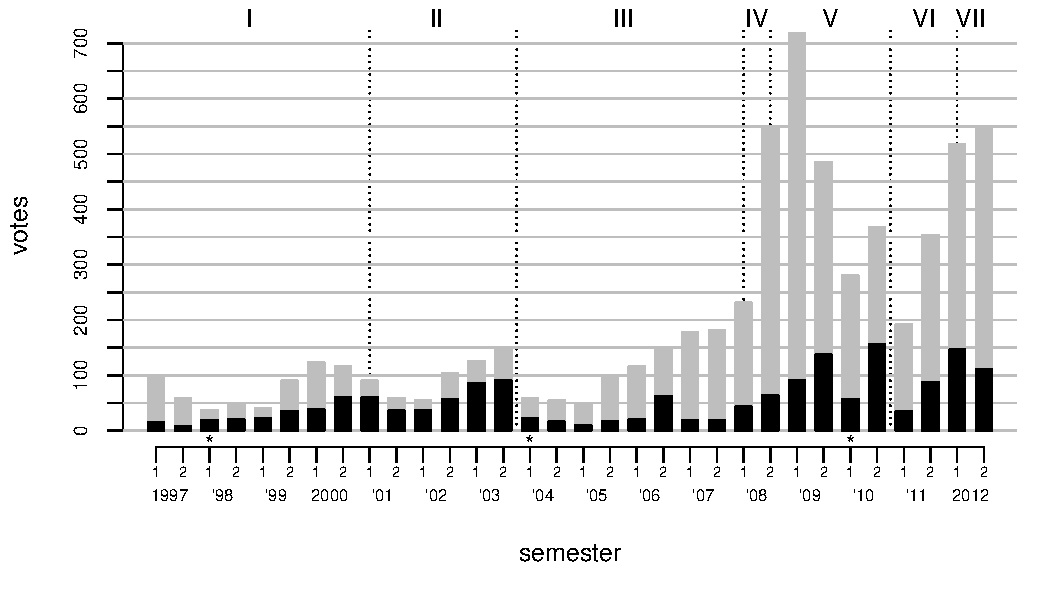
\includegraphics[width=.9\textwidth]{../../graphs/all+divVotsSemester.pdf} \\
    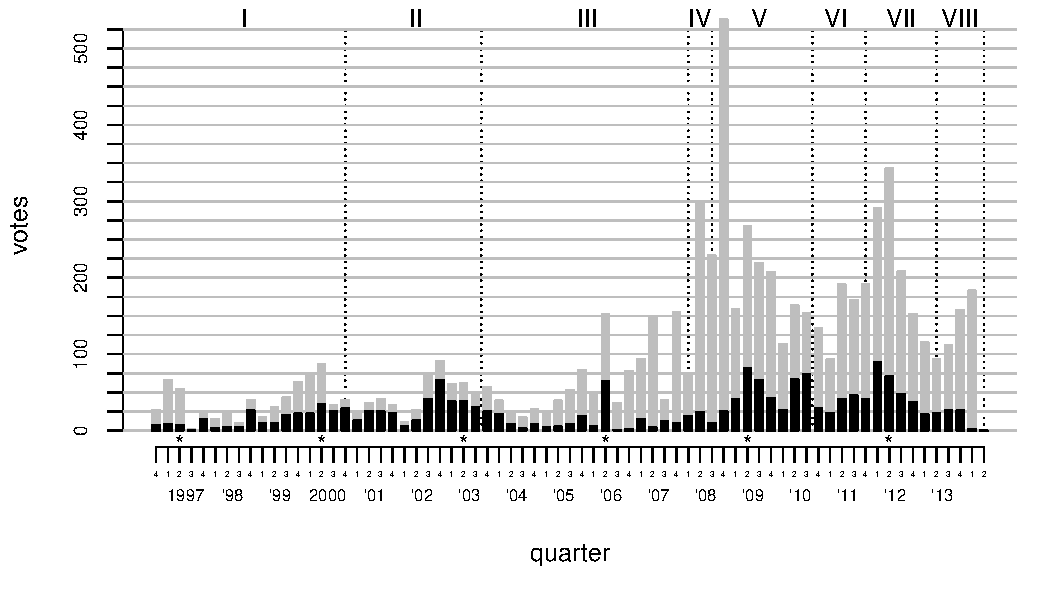
\includegraphics[width=.9\textwidth]{../../graphs/all+divVotsQuarter.pdf} \\
 \caption{\emph{Universe of roll-call votes and analyzed subset.} Grey and black portions of columns indicate unanimous and divided votes in the period, respectively. Dotted lines mark partial or full Council renewals. Periods I and II correspond to Woldenberg's presidency of the Council General, period III to Ugalde's (including Albo's short interim presidency towards the end), and the remainder to the Vald\'es presidency. Stars on the $x$-axis mark federal election quarters.}\label{F:all+div}
 \end{center}
\end{figure}

% Respuesta de Arturo S�nchez a por qu� se dispara n�mero de votos en 2008
% 1. La reforma electoral de ese a�o gener� la necesidad de tomar muchas deciciones:
%   *   Cambios reglamentarios.
%   *   Ajustes a la estructura del Instituto.
%   *   Designaciones de nuevos funcionarios.
%   *   La modificaci�n de las Pol�ticas y Programas del instituto para el proceso de 2009.
%   *   Llegaron nuevos consejeros.
%   *   El Presupuesto y el plan integral del proceso electoral.
% 2. En ese semestre quer�amos terminar con todas las quejas que tra�amos pendientes de a�os anteriores, de manera que el proceso electoral 2008-2009 empezara de cero.
%   *   En una sola sesi�n votamos 56 quejas y 7 acuerdos.
% 3. Recuerda que en octubre de 2008 empezaba el porceso electoral. Ello llevaba en s� mismo un ajuste en materia de preparaci�n, dada la nueva ley. Recuerdo la cantidad de cosas relacionadas con medios de comunicaci�n que ahora ten�amos que votar, incluyendo los tiempos para las elecciones locales.
% 4. Si comparas el n�mero de sesiones del Consejo General, ver�s que en 2007 tuvimnos 14 sesiones en todo el a�o. En el 2008 celebramos 32 sesiones y en el 2009, 96 sesiones. Es l�gico que en este peri�do se hayan incrementado el n�mero de votaciones.

Our goal is to use the information described in Figure~\ref{F:all+div} to obtain estimates of councilor ideal points that change throughout time.  Achieving this goal requires that we address thorny theoretical and methodological problems.  On the theoretical side, the biggest conundrum we face is conveying what dynamic ideal points represent.  In our view, ideal point shifts cannot exclusively represent changing ideological or doctrinal preferences, which seems to be the dominant interpretation of ideal point drift in, for example, studies of the US Supreme Court (Martin and Quinn \citeyear{martin.quinn.2007}; but see Lauderdale and Clark \citeyear{lauderdale.clark.courtManyMedians.2012}). IFE councilors enjoy relatively short appointments, not tenure for life; according to current rules, councilors are appointed for nine years without possibility of renewal. Though it is conceivable that councilors will change their views on electoral regulation during the course of a decade, the amount of drift that we uncover reflects short-term changes in voting behavior.  Dynamic ideal points reveal long-term deep-seated ideological preferences, but are also affected by more permanent changes in coalitional patterns among councilors and by transient changes in the types of issues with which the Council General is forced to grapple. In the next section, we exploit these transient changes in the composition of votes to test some implications of the party watchdog model.

Aside from this basic theoretical conundrum, the estimation of dynamic ideal points presents a panoply of methodological difficulties.  We are aware of two basic approaches to the dynamic estimation of ideal points. The first approach is the dynamic ideal point model used to generate Martin-Quinn scores of the US Supreme Court \citep{martin.quinn.2002}.  In this setting, a separate set of ideal points is estimated each term, but the term-specific ideal point estimates of judges are allowed to ``borrow strength'' from one period to the next. This approach yields dynamic paths with smoothness determined more or less arbitrarily by the researcher and works well in situations where there are many terms and many votes within each term.  In the US Supreme Court, furthermore, turnover among judges is very limited and docket control guarantees that the composition of cases that the Court decides on is the product of selection criteria that do not change drastically from year to year. We cannot afford such luxuries, but we have attempted to mimic this approach in the following way: Rather than considering all votes within a year, we break down the roll call data by trimesters and we impose the condition that the ideal points of councilors follow a random walk (i.e., the ideal point $x_{it}$ of councilor $i$ at time $t$ is informed by her ideal point at time $t-1$, which enters as prior information).  Unfortunately, the number of contentious votes available for estimation varies drastically across quarters, and differences in the sheer volume of available information may determine movements in estimated ideal points that are caused neither by long-term changes in preferences nor by transient shocks.\footnote{We are grateful to Scott Desposato for helping us understand the consequences of variation in the number of bills in the context of a different research project.}

The second approach is the dynamic optimal classification model pioneered by \citet{bonica.dynamicIPs.2009}, which combines a kernel smoothing approach with the OC algorithm of \citet{poole.optimalClassification.2000}. In this approach, ideal points are allowed to vary continuously over periods of very short duration, such as daily sessions.  This assumption suits us well, as it allows the estimation of ideal points that can shift continuously over arbitrarily short periods.  We allow ideal points to potentially change vote by vote.  To identify vote-by-vote ideal points, we carry out as many separate estimations as there are votes in an entire Council General.  For each vote $i$, we base ideal point estimates on all votes captured within a window from vote $i-k$ to vote $i+k$ (we fix $k=15$).\footnote{We initially estimated models with Council session-by-session day-by-day shifts, fixing the number of days in the observation span constant (sessions last one day); this route, however, was also compromised by ample variability in available contentious votes in each session.} Deviating from \citeauthor{bonica.dynamicIPs.2009}'s approach, we estimate IRT rather than OC models in each iteration. We also make a random walk assumption to connect $x_{it}$ to $x_{i,t-1}$.  Compared to the quarter-by-quarter approach that mimics the Martin-Quinn method to obtain Supreme Court dynamic scores, our vote-by-vote estimates are drawn from blocs of information of similar size (except for ideal points at the beginning and at the end, which are estimated on as few as sixteen votes, as the left/right whiskers of the observation window become censored). The vote-by-vote model therefore repeats the estimation for every item, taking some posteriors of the previous estimation as priors. We ran each method for periods I-II and periods III-VII---with fully disjoint memberships---separately. (Day-by-day estimates for periods III-VII is not yet ready in this preliminary report.)

Both estimation methods require the use of informative priors for identification purposes. We use informative priors on the ideal points of councilors to define the polarity of the ideological space. Our choice of priors for the first quarter (or the first vote) of the periods I and III---when the Council General was fully appointed---is based on knowledge of political dynamics at the beginning of these periods drawn from our previous work.\footnote{Models in \citet{estevez.magar.rosas.2008} identified the policy space by resorting to informative priors on a handful of item parameters. Fixing the sign and magnitude of the $\texttt{signal}$ parameter of key votes sets the polarity of the the policy space, portraying Council segmentation in understandable terms. The present work simply recovers information about extremist councilors for space identification purposes.} As we move on through various quarters or votes, we allow the posterior means of each councilor's ideal point distribution to be the prior mean for the next iteration. As new members enter the Council General, the vote-by-vote model uses the the mean of the most recent ideal point estimates for councilors sponsored by the same party as an initial prior. For example, councilor Luken's ideal point as he enters the Council in the last quarter of 2000 is assumed to be identical to the mean of the last estimated ideal points of councilors Molinar (who left the Council) and Lujambio, both PAN-sponsored appointees like the new entrant. The quarterly model, by carrying the optimization exercise once over the full set of divided votes in the period analyzed, demands informative priors for two extremists at the start of the series only for space identification---Councilors Barrag\'an/C\'ardenas and G\'omez Alc\'antar/Gonz\'alez Luna mark the north/south of the I-II and III-VII specters, respectively, in the first quarter in their series. The remaining members can have non-informative priors, although trial-and-error revealed that adding informative priors to a couple of other councilors (Councilors Vald\'es and Figueroa at the south upon their entry) speeds convergence of the MCMC algorithm. 

\begin{figure}
 \begin{center}
%  \begin{tabular}{cc}
%    (a) & (b) \\
   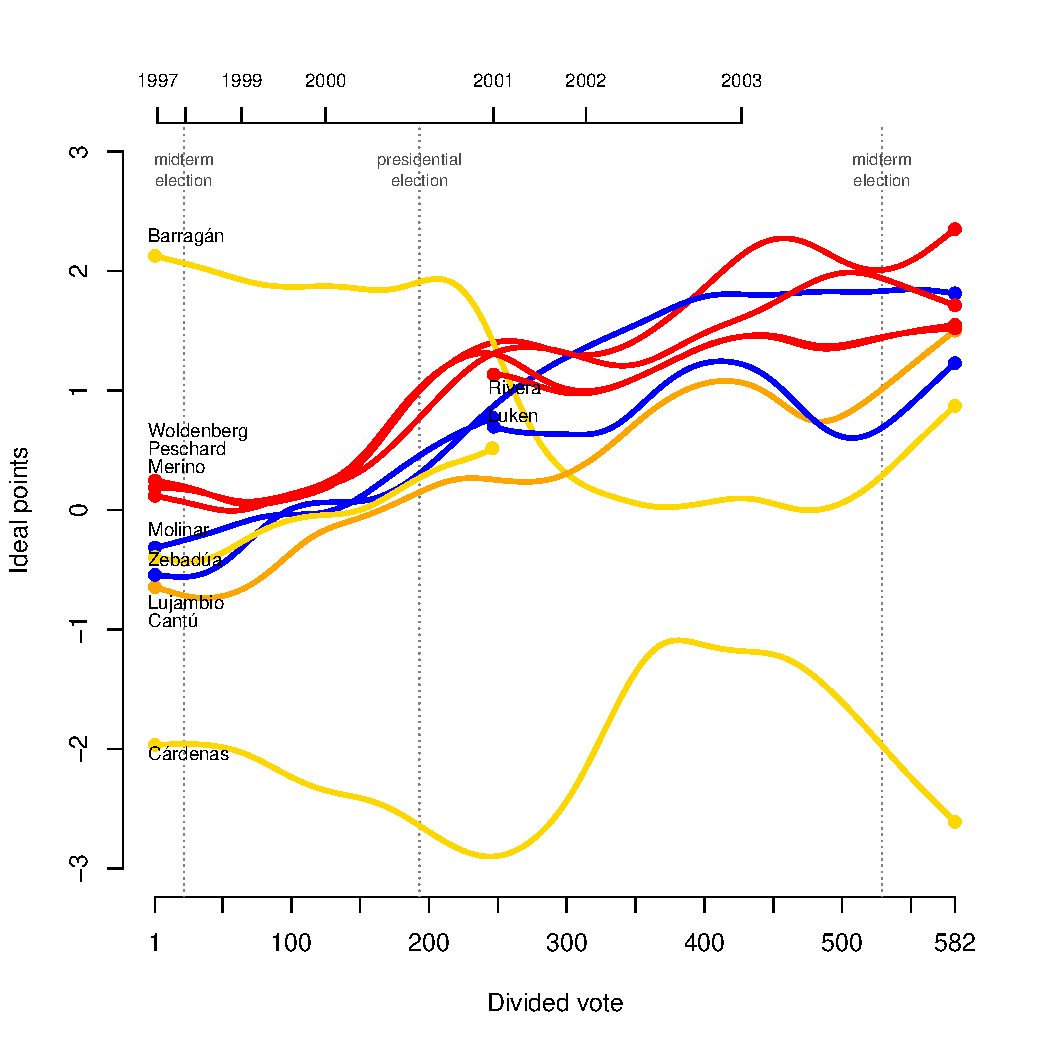
\includegraphics[width=.7\textwidth]{../../graphs/woldBonicaSmoothLines.pdf} %&
%    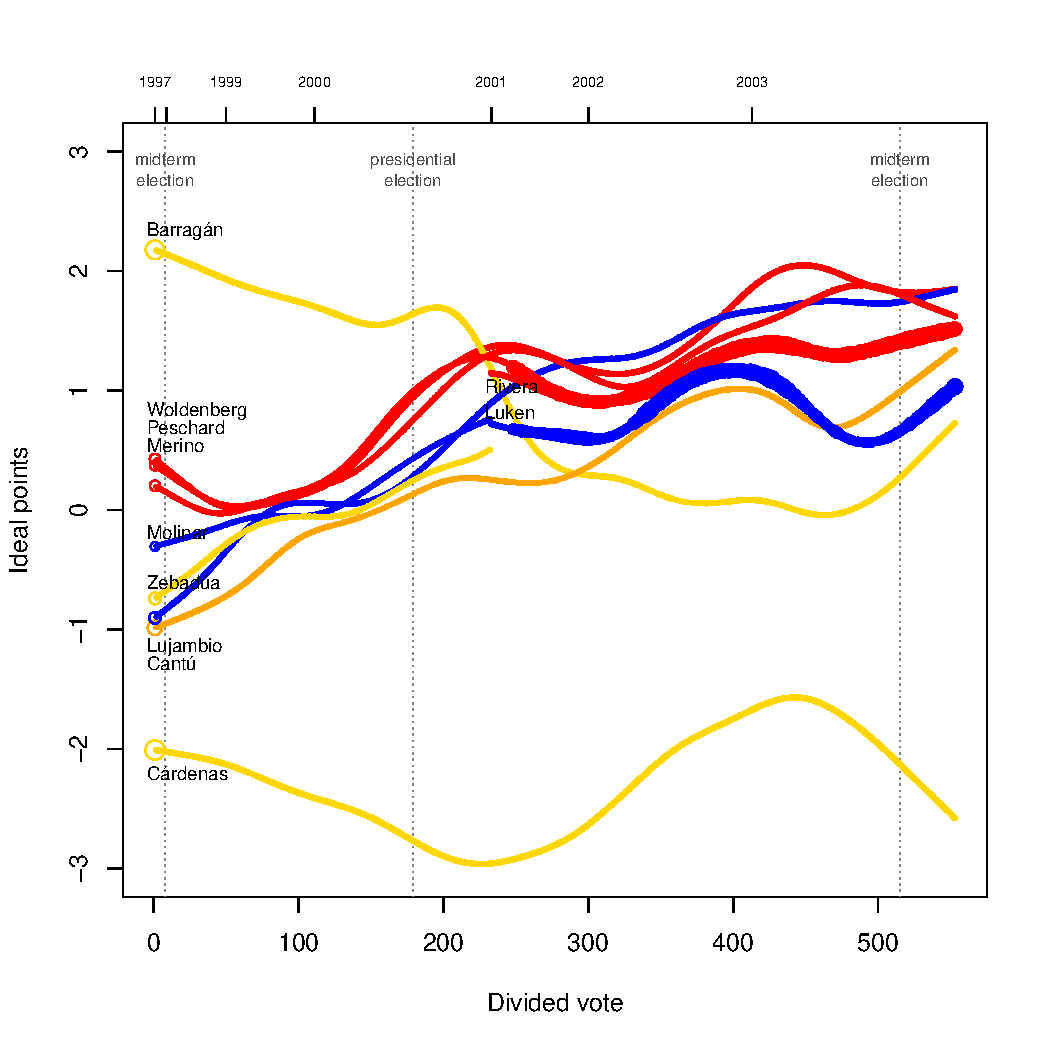
\includegraphics[width=.48\textwidth]{../../graphs/woldBonicaSmoothError.pdf} \\
%  \end{tabular}
  \caption{\emph{The Woldenberg Council.} Lines report the median of each councilor's posterior density, colors indicate councilor's sponsoring party: blue = PAN, red = PRI, gold = PRD, orange = PRD--PT.}\label{F:spaghettis}
 \end{center}
\end{figure}

Figures~\ref{F:spaghettis} and~\ref{F:spaghettis2} present results of the dynamic ideal point models of Martin-Quinn and Bonica, respectively.  Our first task is to assess the face validity of these plots.  This task is easier for the two Woldenberg councils (1996--2003) on account of the amount of anecdotal information that we have collected over the years.  The most obvious pattern emerging from Figure~\ref{F:spaghettis} and the leftmost plot of Figure~\ref{F:spaghettis2} is the gradual formation of a voting bloc comprising PAN- and PRI-sponsored councilors toward the end of 2003; the formation of this bloc is all the more surprising  given that PAN- and PRI-sponsored councilors had often opposed each other in a number of decisions up until 1997.

\begin{figure}
 \begin{center}
  \begin{tabular}{cc}
    (a) & (b) \\
    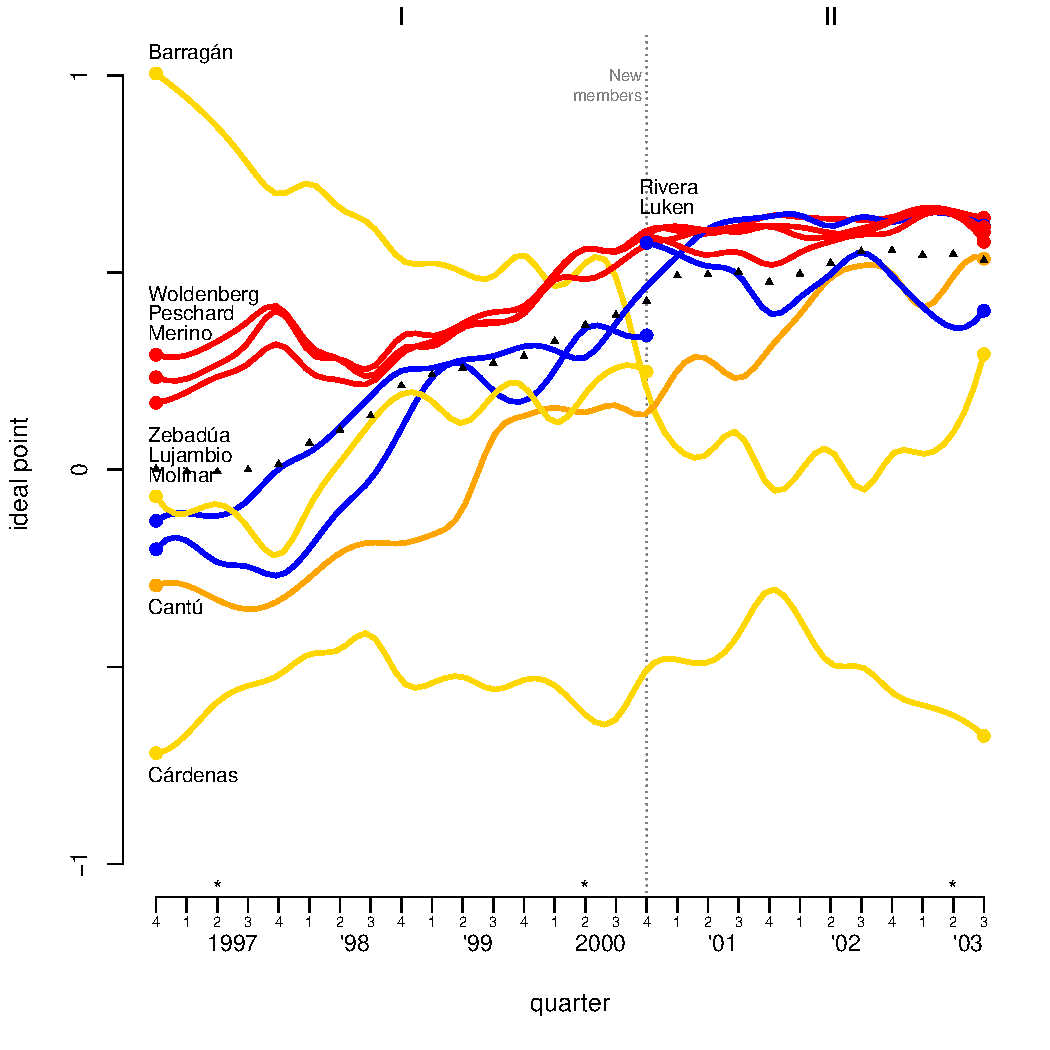
\includegraphics[width=.48\textwidth]{../../graphs/allWdynQuarter.pdf} &
    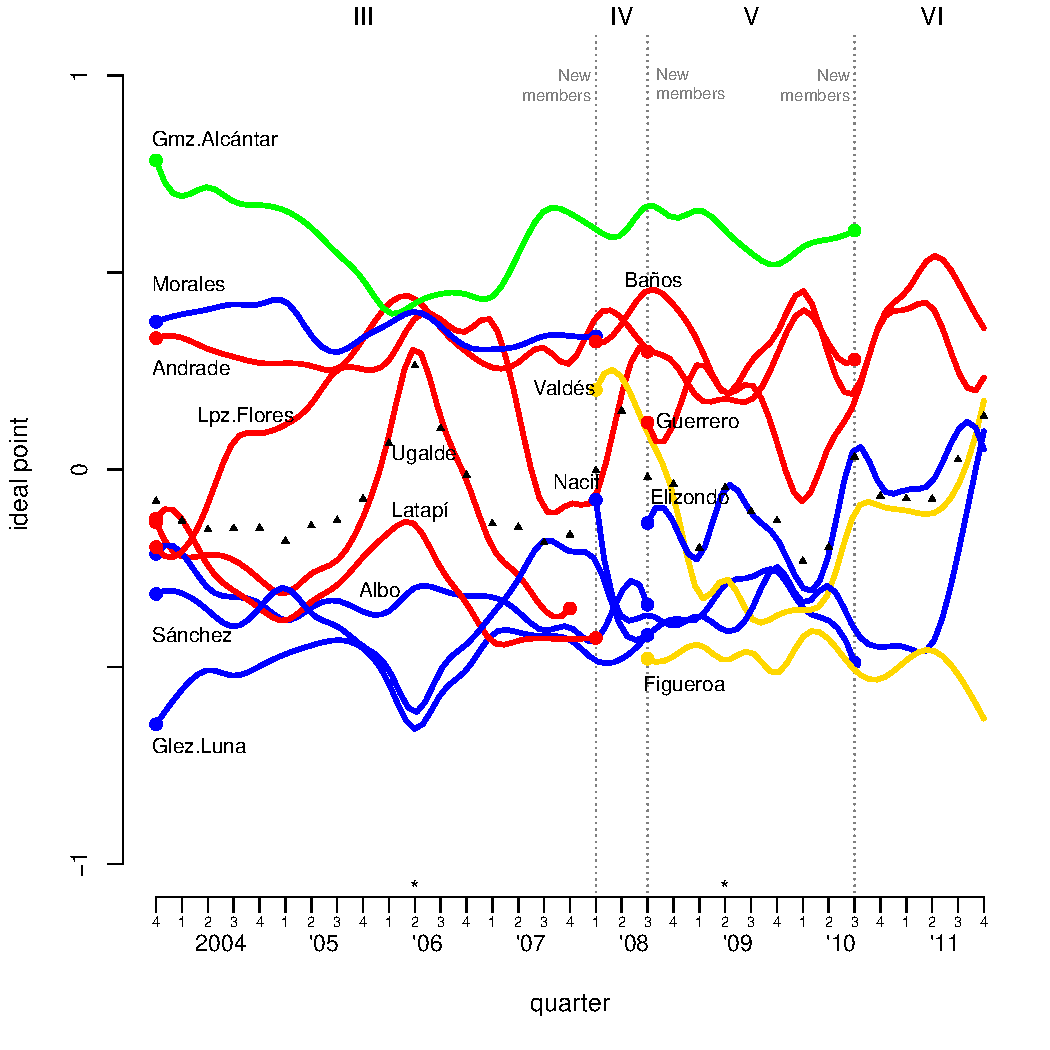
\includegraphics[width=.48\textwidth]{../../graphs/allUAVdynQuarter.pdf} \\
  \end{tabular}
  \caption{\emph{Six Councils General.} Lines report the median of each councilor's posterior density, colors indicate councilor's sponsoring party: blue = PAN, red = PRI, gold = PRD, orange = PRD--PT, green = Green. Triangles report expected council median. Stars in x-axis mark federal election quarters.}\label{F:spaghettis2}
 \end{center}
\end{figure}

Let us focus on an account of the creation of a supermajority voting bloc, and particularly on Councilor Lujambio's flanking movement.  Councilor Lujambio, committee chair for campaign and party finance regulation, was in charge after the 1997 midterm elections of assessing fines on political parties for campaign misconduct. After separate committee resolutions for each political party were negotiated and shepherded through council approval, all affected parties appealed the council decisions to the electoral tribunal, which overruled or amended the council's decisions in all but one case. Never again did Lujambio's committee issue separate reports on the parties, but instead logrolled them into a single resolution requiring an up-or-down vote on the council.

The following year, the committee had to review non-electoral party revenues and expenditures, but Lujambio found that the other members of his committee (two colleagues sponsored by the PRI) hesitated in following Lujambio's proposal to levy fines, arguing that they could not ignore the electoral tribunal's criteria from previous rulings. Several months passed before the reports could be issued, and only after Lujambio had lobbied tribunal judges exhaustively.  He would conduct similarly intensive lobbying with the judges until his term ended in 2003, but continued resistance by the other committee members would be met with a singular innovation which Lujambio proposed and obtained in 1999 from the Council General.  Committee membership was to be expanded to include \emph{all} members of the council except the president, thus saving the original committee members from intense pressures from their party sponsors whenever they had to levy fines.  

The council as a whole was quite willing to acknowledge the growing expertise of Lujambio and his staff in this crucial field of electoral regulation and to delegate these matters to them.  In return, Lujambio, having started his tenure in opposition to councilors sponsored by the PRI and in alliance with a crew of councilors informally known as \emph{el Pent\'agono}, quickly moved after 1999 to join a cohesive and durable majority with PRI-sponsored councilors.  He followed the paths trailblazed by Molinar and Zebad\'ua three or four quarters before, and was himself later followed by Cant\'u, seeking similar council support for his initiatives as committee chair for electoral organization.  The PAN contingent moved practically in tandem to leave behind the \emph{Pent\'agono} alliance and join the PRI contingent in majority control of the council. Just as impressive was the ``northbound'' migration of two councilors sponsored by the leftist PRD, Zebad\'ua and Cant\'u.

A second anecdote places in context our discovery of the slow formation of a supermajority in the latter half of Woldenberg's Council.  The key to the development of this super-majority in 1999 was the decision taken by Woldenberg himself and supported by the rest of his contingent to back the ouster of Felipe Sol\'is as Secretary-General of IFE's bureaucracy.  Woldenberg had been supported by the PRI for the Council President post as part of a ticket including the appointment of Sol\'is as the council's first major decision.  Woldenberg and the council duly complied with the prearranged appointment.  After matters pending from the 1997 midterms had been wrapped up, members of the \emph{Pent\'agono} began to pressure Woldenberg and his contingent for a break with IFE's administrative past.  Sol\'is had been a lieutenant to IFE's first Secretary-General in 1990, Emilio Chuayffet, then and now a top politician within the national PRI (and after leaving IFE, Sol\'is would go on to elective federal posts in Congress and to positions in the PRI's national directorate).  Autonomy of the electoral authority, argued the \emph{Pent\'agono}, could only be assured if the council took direct control over the administrative officers of its bureaucracy and permitted the Council's committee system to exercise strong oversight over IFE's operational areas.  Woldenberg and his contingent resisted these appeals, until the Comptroller, another PRI stalwart, unexpectedly filed administrative complaints against four of the five members of the \emph{Pent\'agono} (these briefs are a legal prelude to possible impeachment by Congress).  Within twenty-four hours, the comptroller was dismissed by the council, at Woldenberg's request, and the complaints rescinded.  It took only a few more months for Sol\'is to tender his resignation.  

This forthright commitment by Woldenberg to IFE's autonomy made all the difference, and paved the way toward the creation of a solid bloc of councilors circling the wagon to protect themselves, and their decisions, from blatant partisan intervention.  Had this not occurred, the Woldenberg council might well have continued to exhibit the fractiousness and instability of its first quarters, despite very high levels of unanimous decision-making, conditions which have also characterized the Ugalde and Vald\'es councils. Unfortunately, without the presence of the former ruling party deep in the entrails of IFE's apparatus, which at one point fostered fiercely defensive unity on the council, the tripartite organization of the Council General itself has imposed the more consistently partisan skew upon its proceedings that now passes for ``normal politics'' at IFE.

\section{Further testable implications of the party watchdog model}
\label{S:hypotheses}

We estimate dynamic ideal points in an effort to validate a number of implications derived from the party watchdog model.  In particular, we focus on three implications: (i) concomitant drift among same-sponsor councilors, (ii) increases in the divisiveness of decisions considered during electoral periods, and (iii) increases in within-contingent coherence and between-contingent polarization during electoral periods.  We proceed now to relate the logic behind each of these implications, as well as the evidence that we have collected to substantiate them.

\subsection{Concomitant drift among same-sponsor councilors}

%The demise of the Ugalde council in the wake of the 2007 reform is an example of resort to the ``nuclear option'' that legislative parties can deploy against IFE's council.  Since IFE's establishment in 1990, four complete sets of councilors have been appointed by Congress (in 1990, 1994, 1996 and 2003).  Of these four sets, two have suffered abrupt and total replacement and another has had two thirds of its membership prematurely ousted. Only the Woldenberg council finished its full term unscathed by congressional interference, although impeachment threats were frequently voiced by leaders and spokespersons of several parties. The not so unusual resort to the nuclear option is the final, ex post instrument used to cow IFE councilors into alignment with their party sponsors.

When moving to a dynamic view of voting in the Council General, the most obvious implication of the party watchdog model concerns the expectation that, to the extent that rearrangements of relative ideal points take place, councilors that were sponsored by the same party should move more or less in tandem.  If, as we believe, political parties vet their nominees thoroughly and if they threaten councilors with early termination, councilors will be less likely to oppose directly the interests of their sponsors.\footnote{
		The demise of the Ugalde council in the wake of the 2007 reform is an example of resort to the ``nuclear option'' that legislative parties can deploy against IFE's council.  Since IFE's establishment in 1990, four complete sets of councilors have been appointed by Congress (in 1990, 1994, 1996 and 2003).  Of these four sets, two have suffered abrupt and total replacement and another has had two thirds of its membership prematurely ousted. Only the Woldenberg council finished its full term unscathed by congressional interference, although impeachment threats were frequently voiced by leaders and spokespersons of several parties.}
The ombusdman view, on the contrary, would not expect councilors' ideal points to move together.

\begin{figure}
 \begin{center}
  \begin{tabular}{ccc}
    (a) 1996--2003 & (b) 1996--2003 & (c) 1996--2003\\
    PAN & PRI & Left\\
    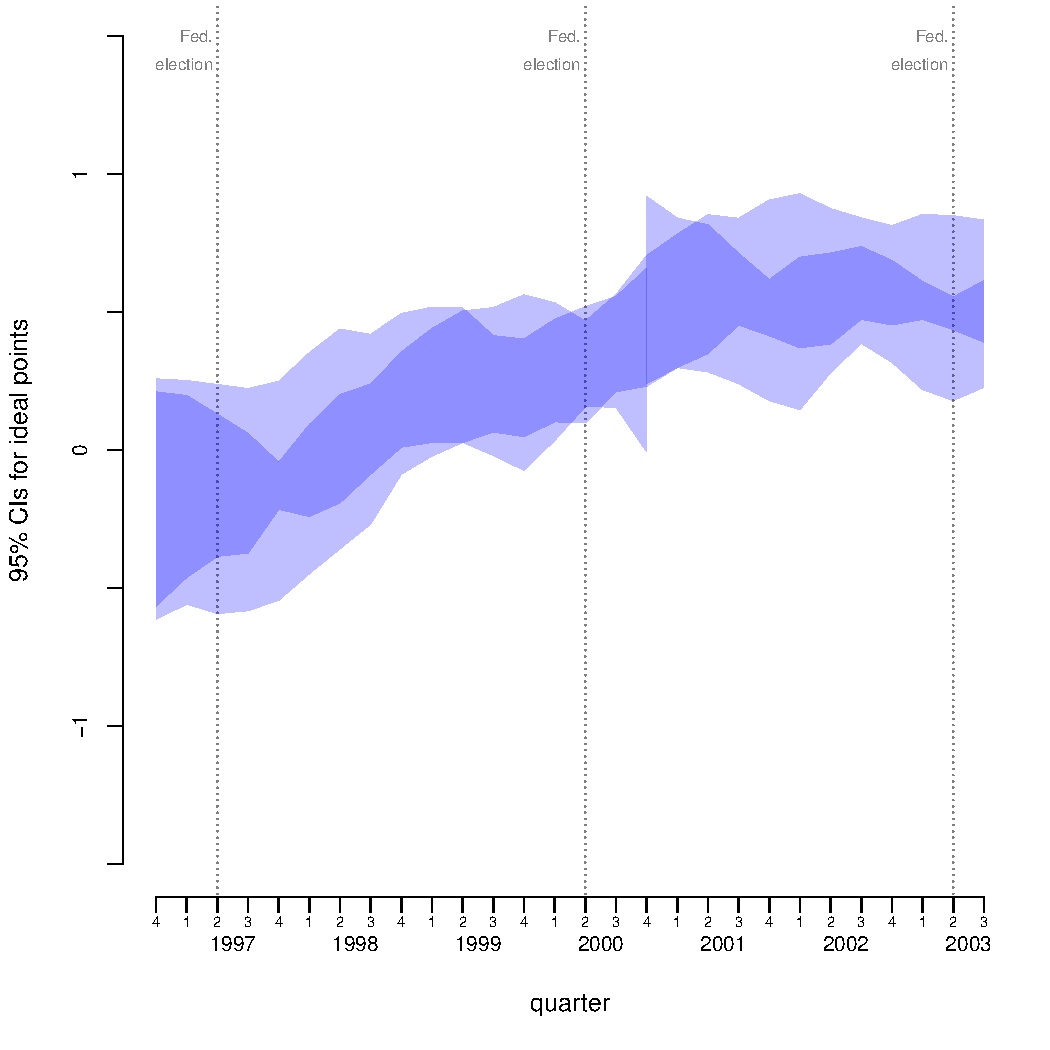
\includegraphics[width=.3\textwidth]{../../graphs/woldStackMartinQuinnQuarterPan.pdf} &
    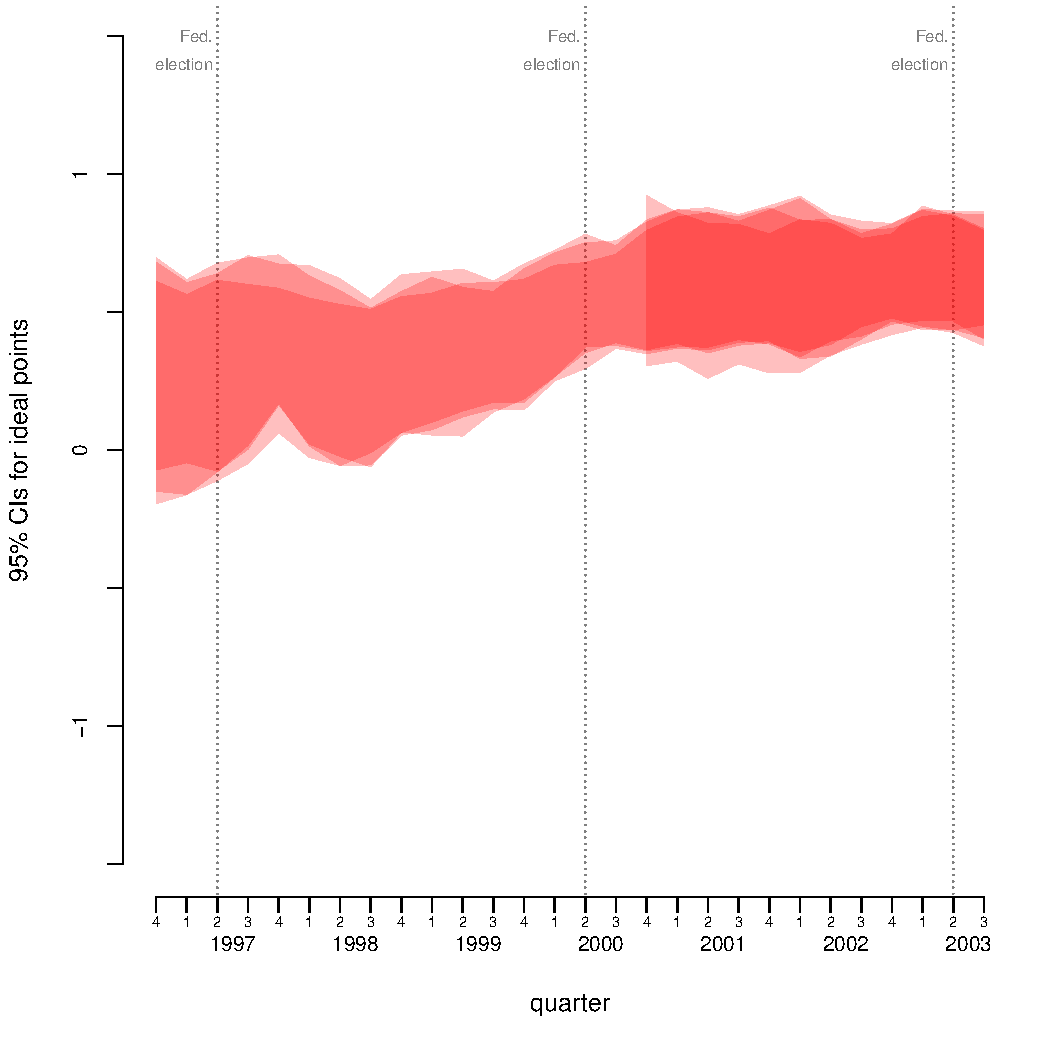
\includegraphics[width=.3\textwidth]{../../graphs/woldStackMartinQuinnQuarterPri.pdf} &
    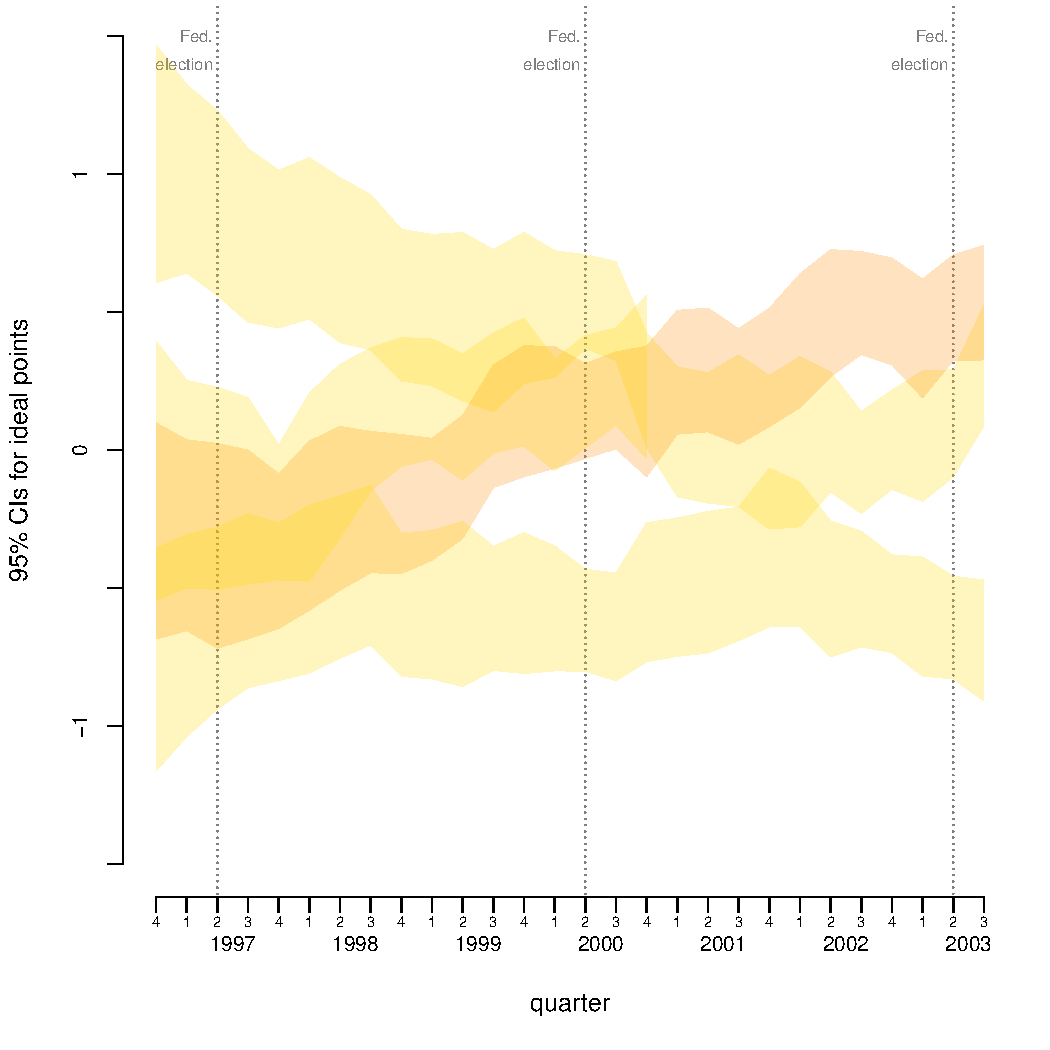
\includegraphics[width=.3\textwidth]{../../graphs/woldStackMartinQuinnQuarterLeft.pdf} \\
    % 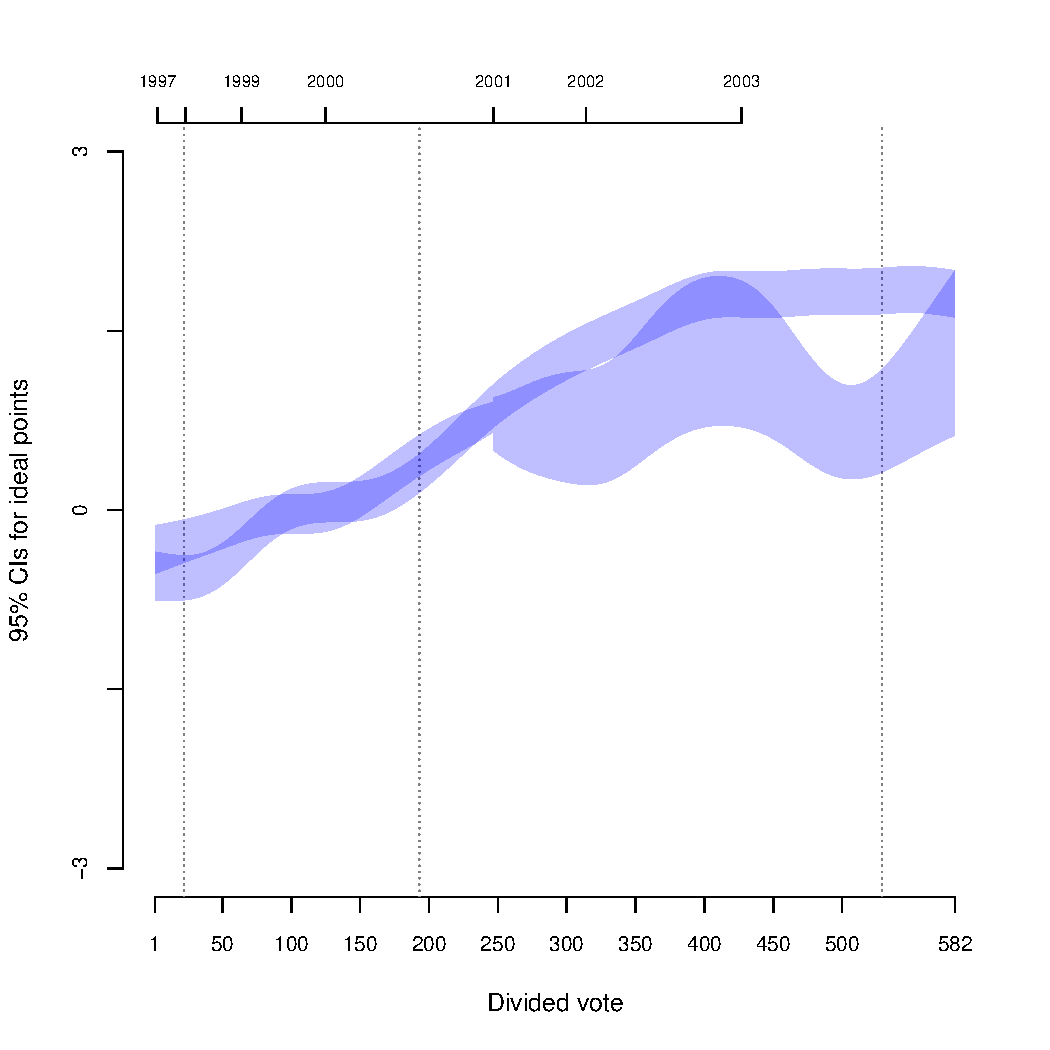
\includegraphics[width=.3\textwidth]{../../graphs/woldStackBonicaPan.pdf} &
    % 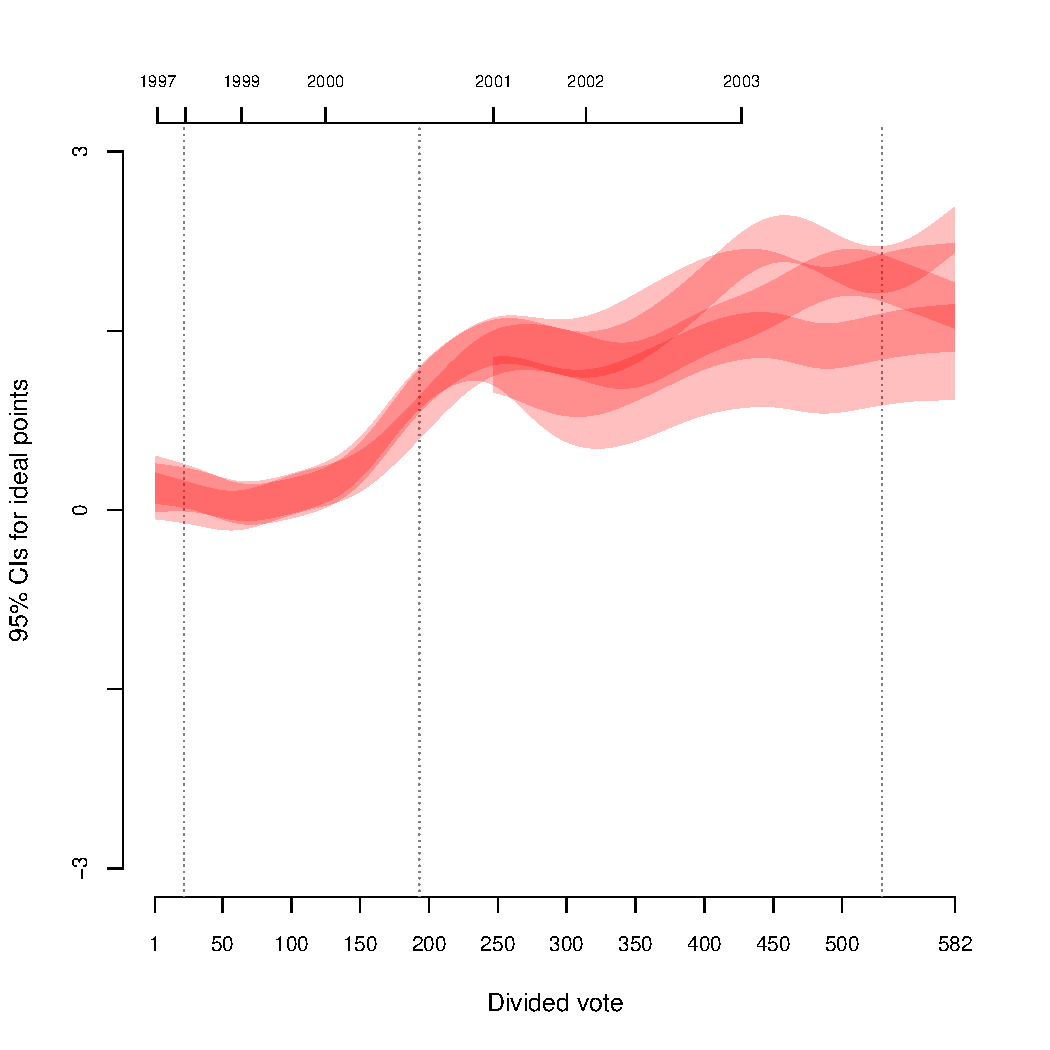
\includegraphics[width=.3\textwidth]{../../graphs/woldStackBonicaPri.pdf} &
    % 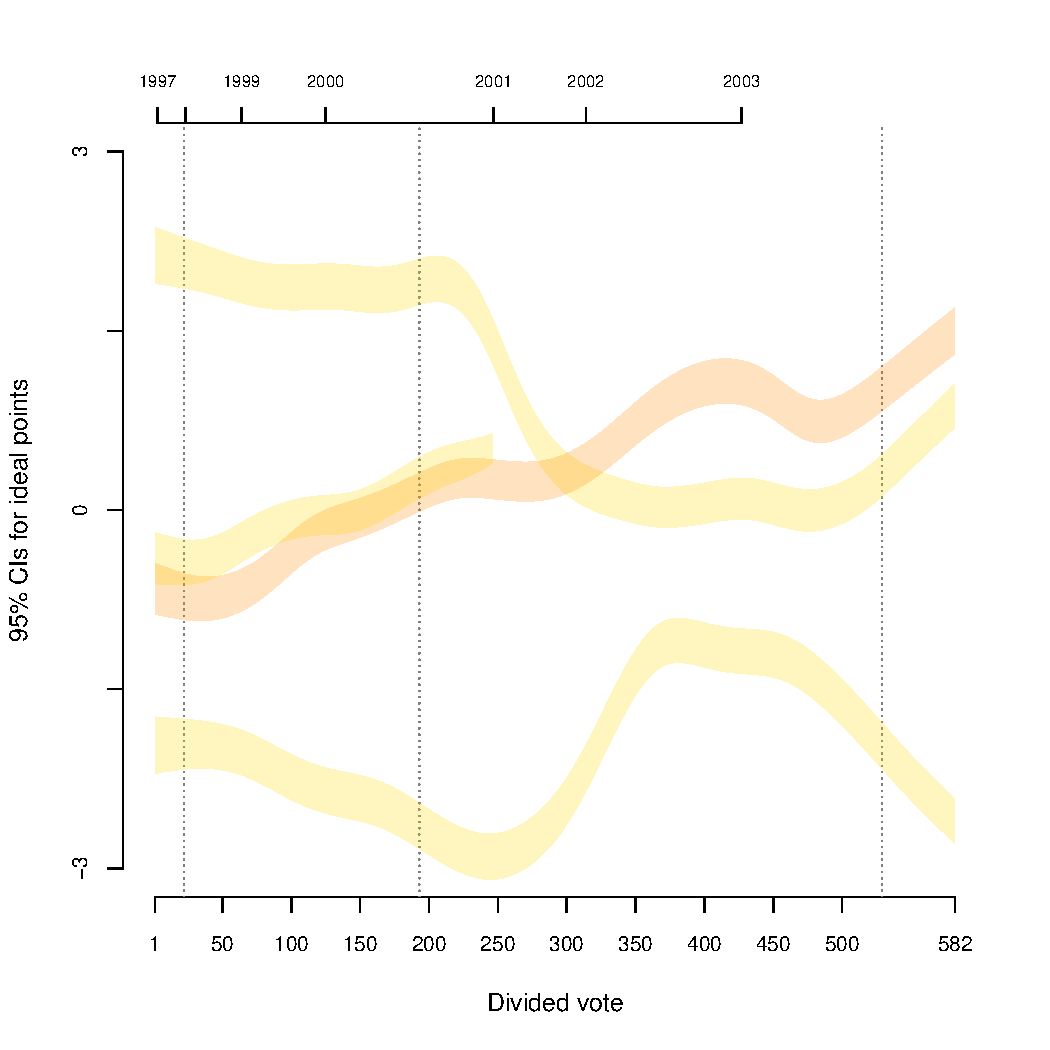
\includegraphics[width=.3\textwidth]{../../graphs/woldStackBonicaLeft.pdf} \\
    (d) 2003--2011 & (e) 2003--2011 & (f) 2003--2011\\
    PAN & PRI & Left \\
    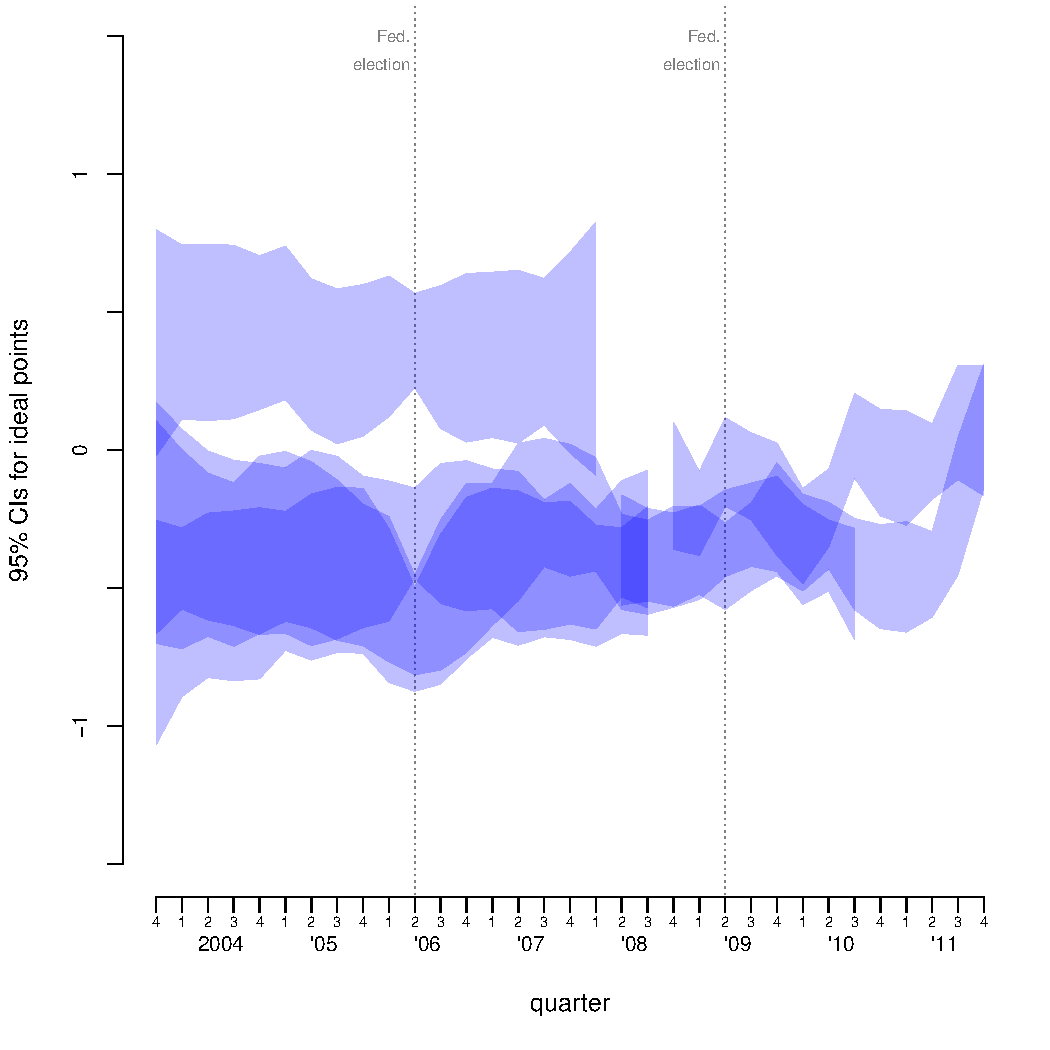
\includegraphics[width=.3\textwidth]{../../graphs/uavStackMartinQuinnQuarterPan.pdf} &
    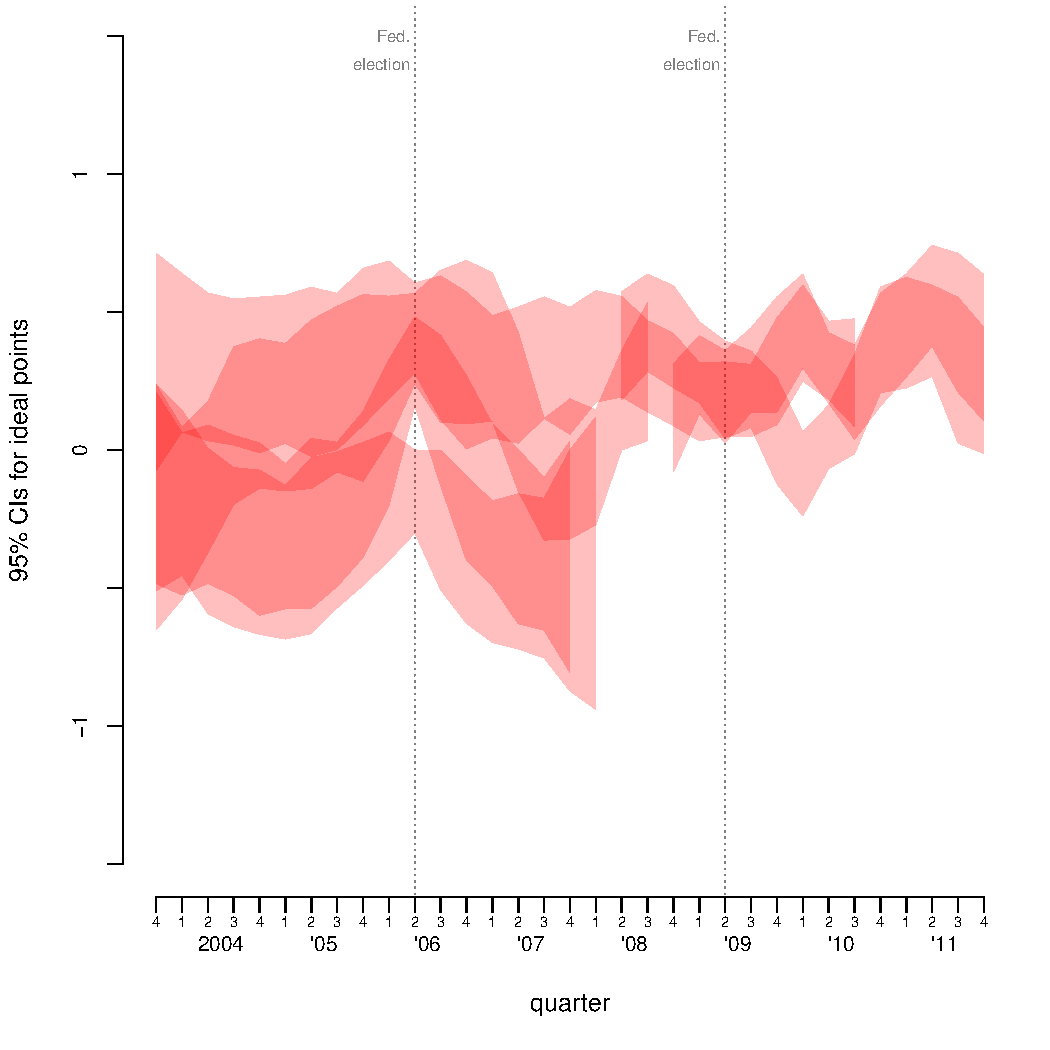
\includegraphics[width=.3\textwidth]{../../graphs/uavStackMartinQuinnQuarterPri.pdf} &
    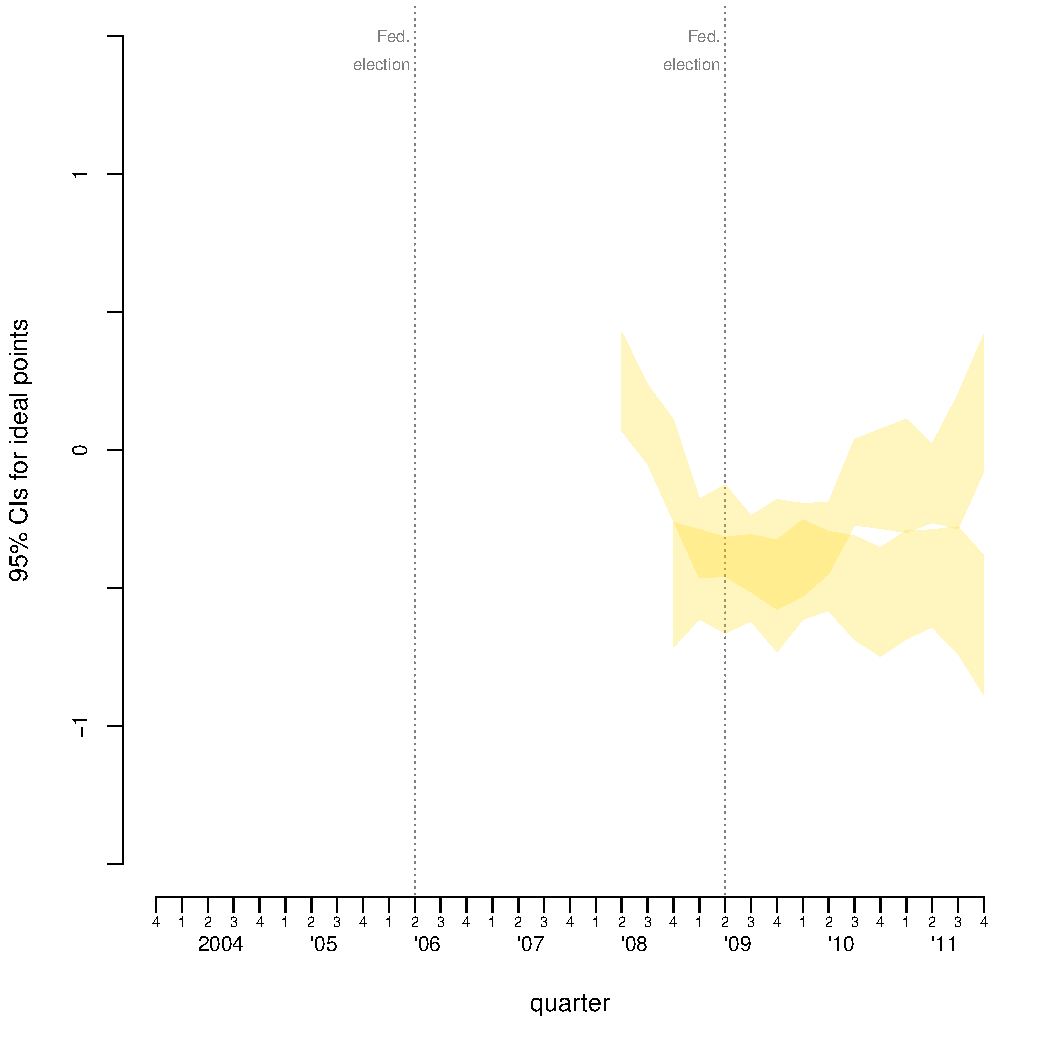
\includegraphics[width=.3\textwidth]{../../graphs/uavStackMartinQuinnQuarterLeft.pdf} \\
    (g) 2003--2011 & (h) 2003--2011 & \\
    PAN-Elba & Green-Madrazo & \\
    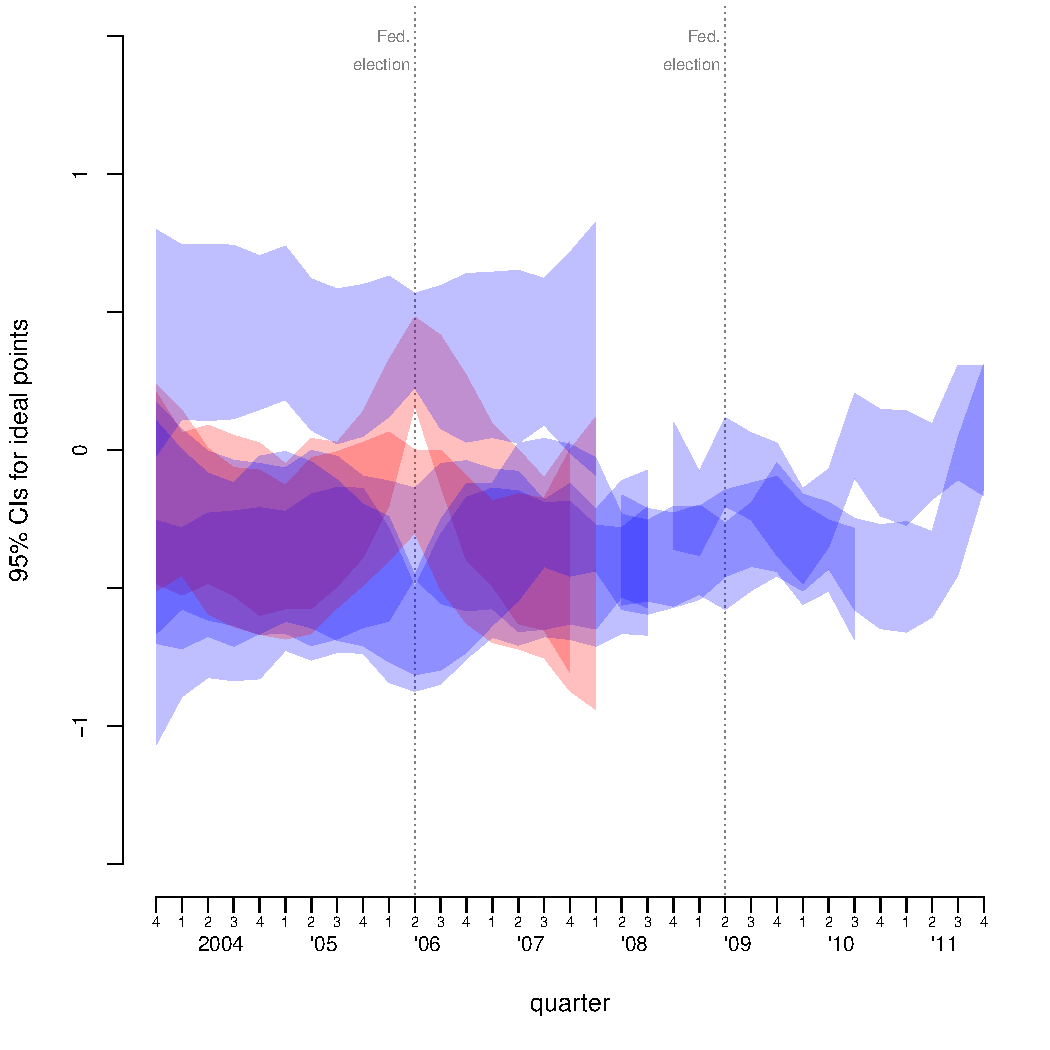
\includegraphics[width=.3\textwidth]{../../graphs/uavStackMartinQuinnQuarterPanElba.pdf} &
    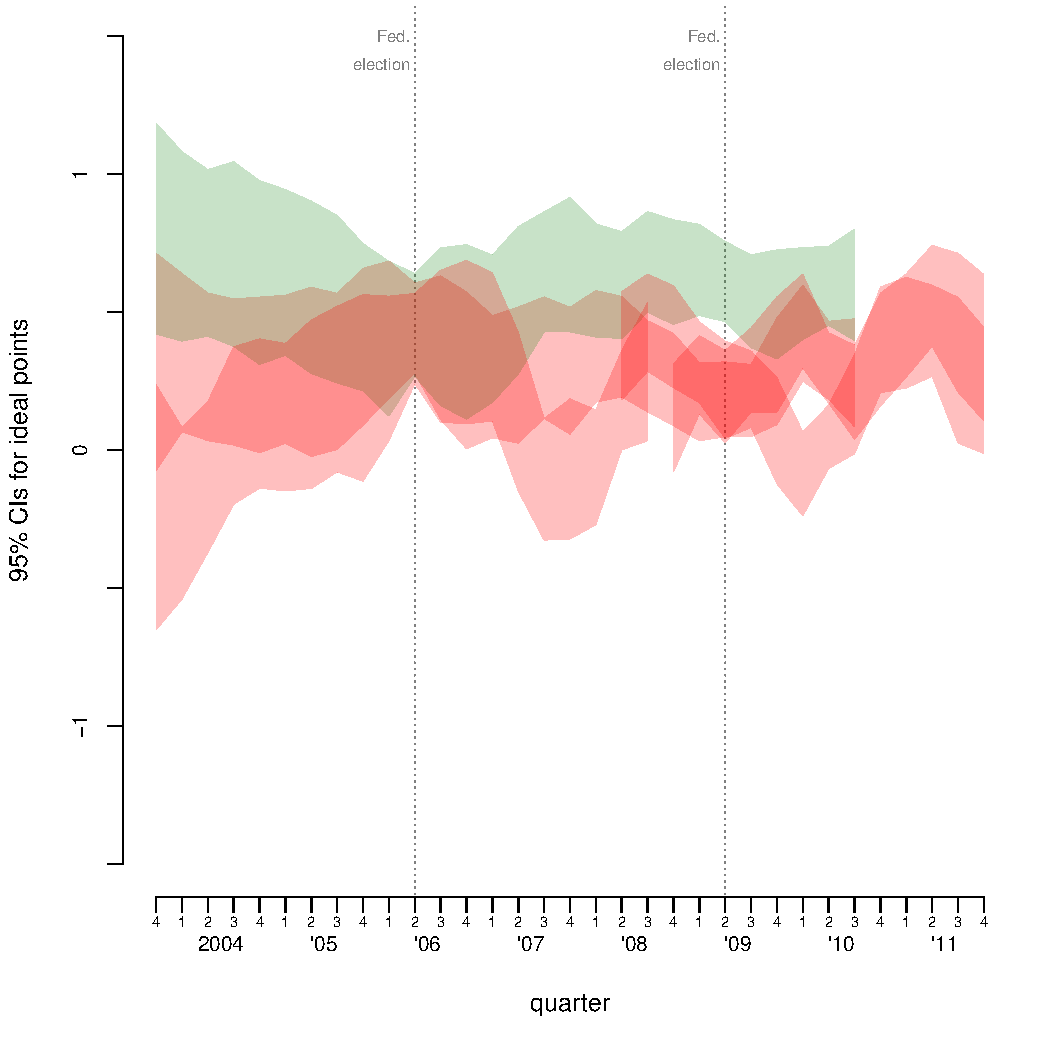
\includegraphics[width=.3\textwidth]{../../graphs/uavStackMartinQuinnQuarterPriMadPvem.pdf} & \\
  \end{tabular}
 \caption{\emph{Overlapping ideal point ranges, quarter-by-quarter model.} Panels report 95\% credible intervals for the ideal points of councilors with a given sponsor.}\label{F:overlap}
 \end{center}
\end{figure}

\begin{figure}
 \begin{center}
  \begin{tabular}{ccc}
    \mc{3}{c}{} \\
    (a) Vote-by-vote & (b) Vote-by-vote & (c) Vote-by-vote\\
    PAN & PRI & Left\\
    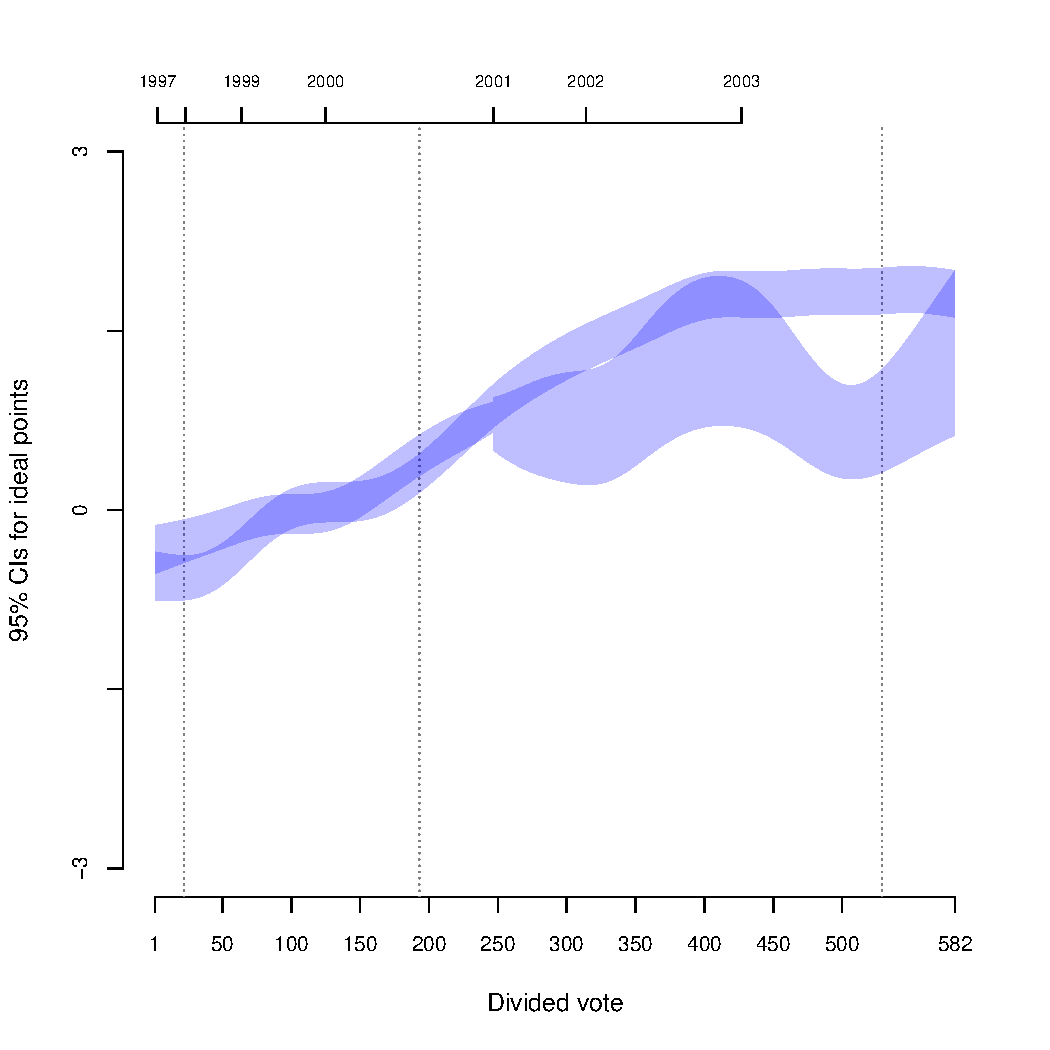
\includegraphics[width=.3\textwidth]{../../graphs/woldStackBonicaPan.pdf} &
    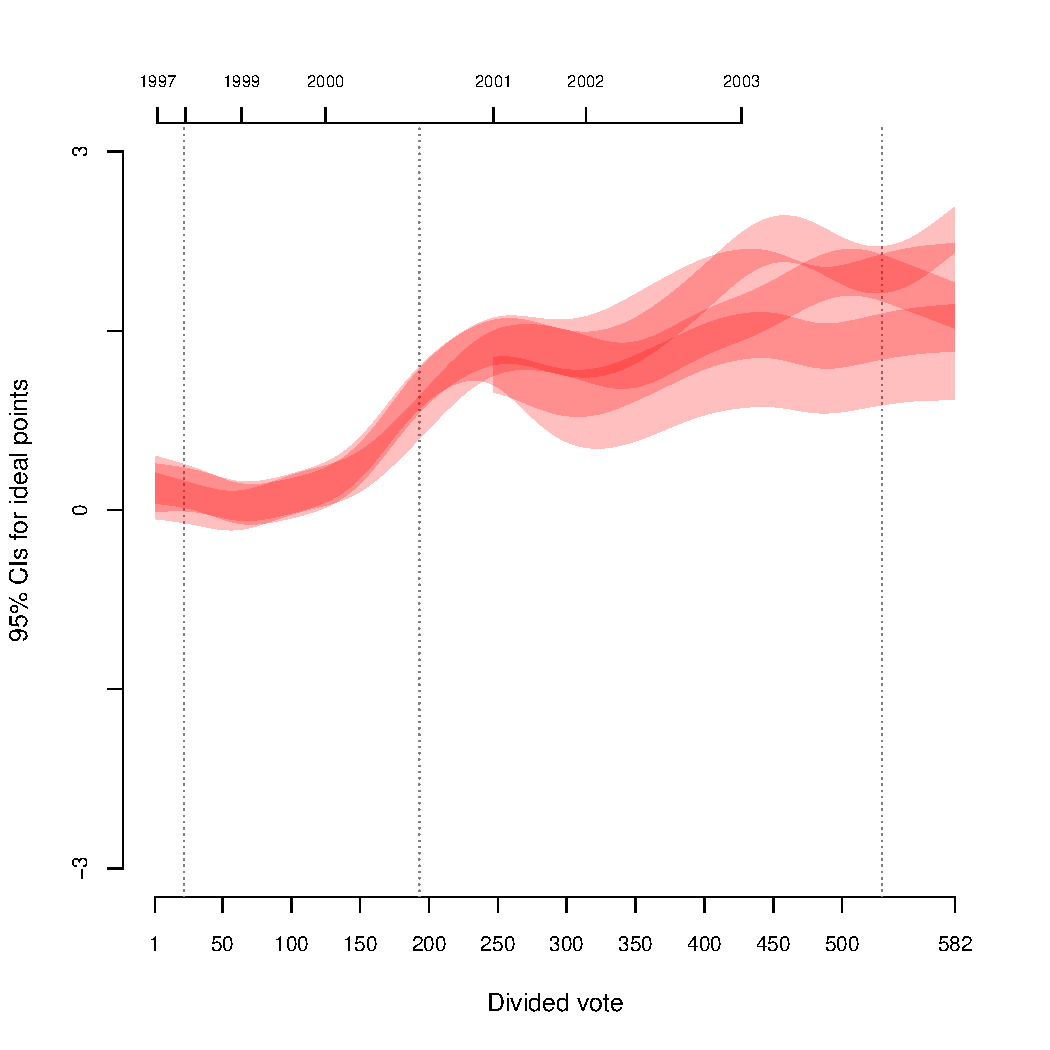
\includegraphics[width=.3\textwidth]{../../graphs/woldStackBonicaPri.pdf} &
    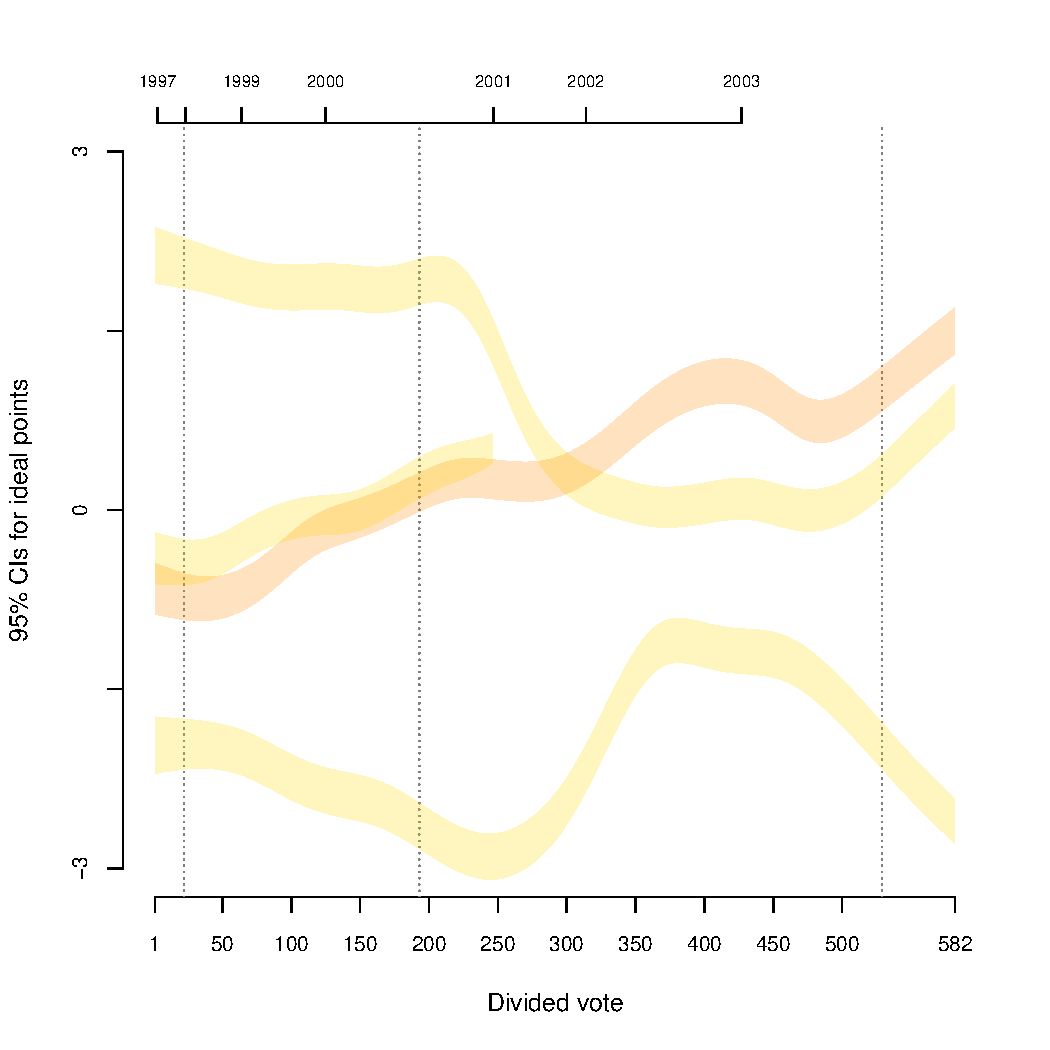
\includegraphics[width=.3\textwidth]{../../graphs/woldStackBonicaLeft.pdf} \\
    \mc{3}{c}{} \\
    (d) Quarter-by-quarter & (e) Quarter-by-quarter & (f) Quarter-by-quarter\\
    PAN & PRI & Left \\
    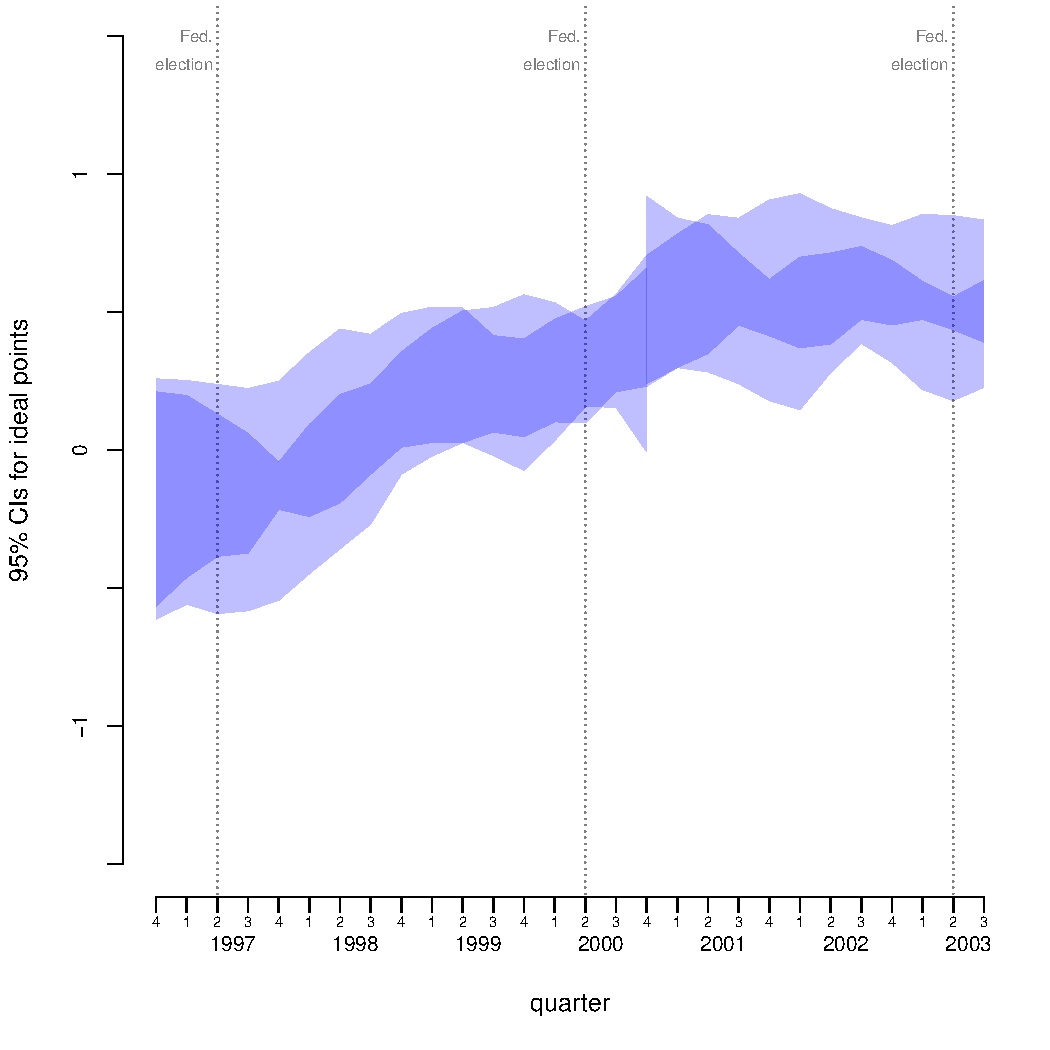
\includegraphics[width=.3\textwidth]{../../graphs/woldStackMartinQuinnQuarterPan.pdf} &
    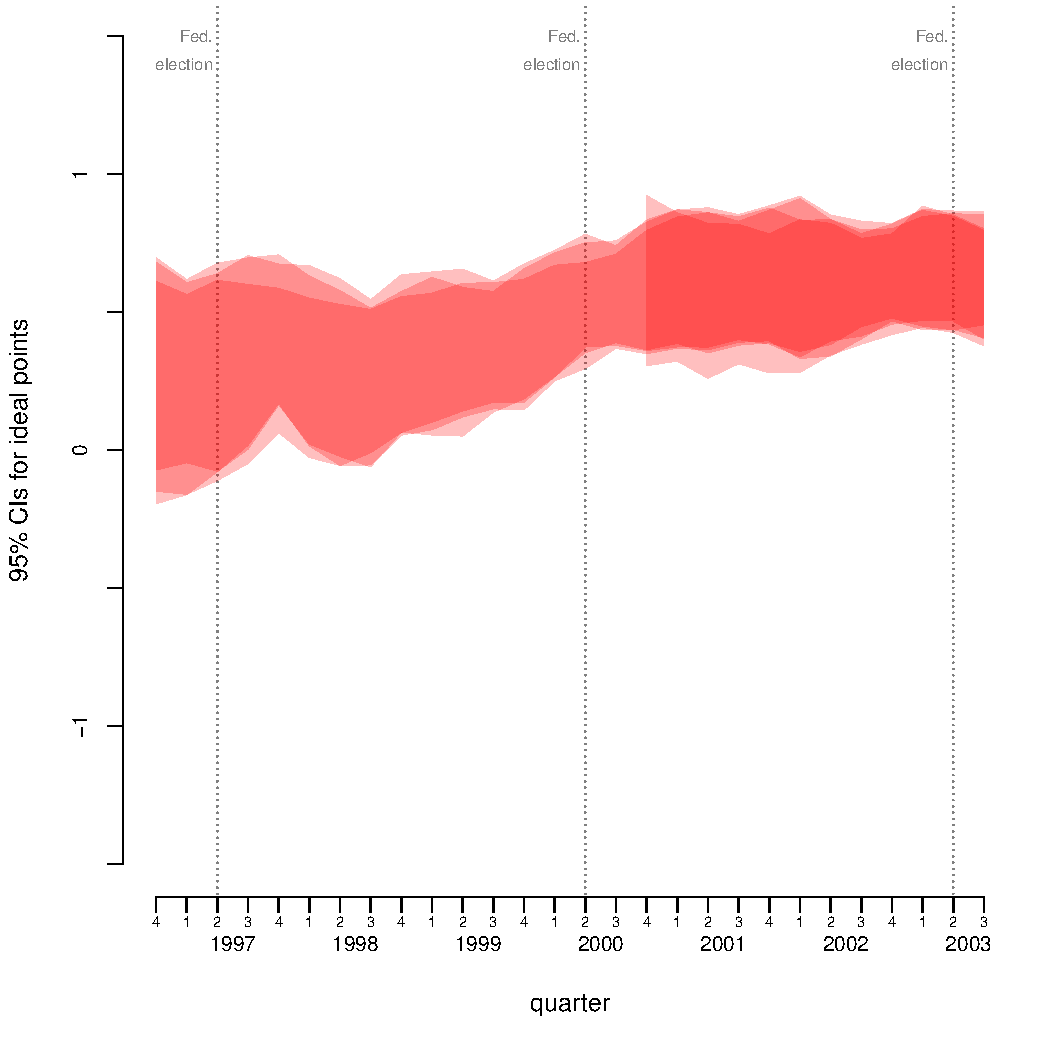
\includegraphics[width=.3\textwidth]{../../graphs/woldStackMartinQuinnQuarterPri.pdf} &
    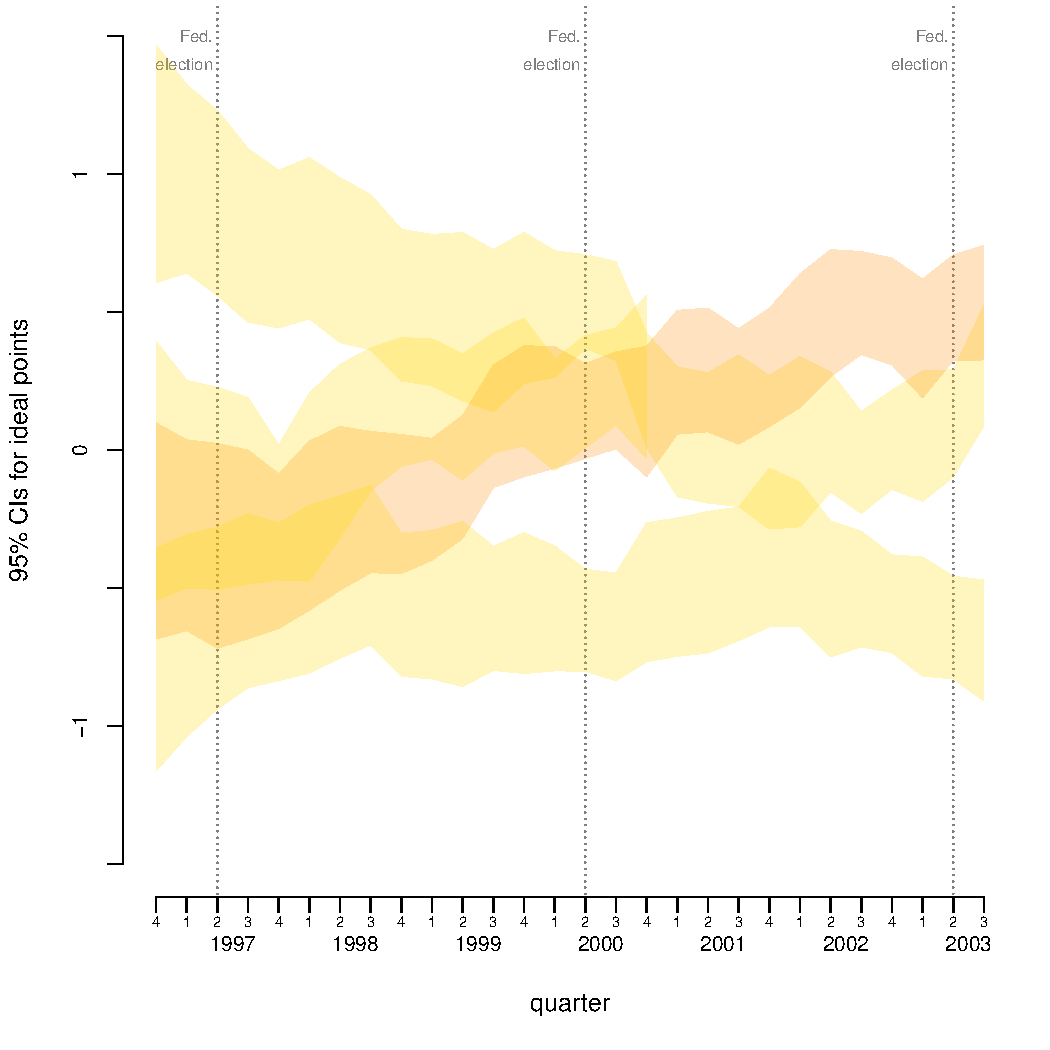
\includegraphics[width=.3\textwidth]{../../graphs/woldStackMartinQuinnQuarterLeft.pdf} \\
  \end{tabular}
 \caption{\emph{Overlapping ideal point ranges 1996--2003 from two models.} Panels report 95\% credible intervals for the ideal points of councilors with a given sponsor, vote-by-vote model and quarter-by-quarter models in the top and bottom rows, respectively.}\label{F:overlap2}
 \end{center}
\end{figure}

Evidence of concomitant drift appears in Figure \ref{F:overlap}, which maps the degree of overlap in ideal point ranges (bands include 95 percent of posterior ideal point samples from the quarterly estimations) over time among multi-member partisan contingents. Alignment in the Woldenberg council (panels a--c) is consistently strong for the PAN's and PRI's contingents before the partial turnover in both of their memberships in 2000. The drift that characterizes PAN-sponsored Councilors Molinar and Lujambio is clear and signals the  \emph{Pent\'agono} breakup. The blue northern migration was slightly less acute for new entrant Luken (panel a). This is more visible in Figure \ref{F:overlap2}a, which allows comparison of cohort confidence ranges obtained with thw two estimation techniques. Luken's voting behavior is somewhat erratic, which widens his ideal point range (the other wider bar after the partial replacement in Figure \ref{F:overlap2}b corresponds to Councilor Peschard). While, in general, Luken remained in the northern half of space, southern pulls towards members of the left are evident around votes 300 and 500, leaving a small gap with co-partisan Lujambio's trajectory. Stacking is inexistent for the Left's contingent (panel c). Most left-sponsored councilors (and, after 2000, all of them) stayed to the south of other contingents, but there was no voting coalescence among all of them at any time in the seven years this council lasted. The early emergence of opposing extremists from the same contingent surely doomed it to eventual insignificance, but the northern drift of Zebad\'ua and, more notably, Cant\'u, while making them players in Council General bargaining also hurt prospects for cohesion of PRD-sponsored councilors.

For the Ugalde, Albo, and Vald\'es councils (panels d--h), the evidence points to  greater stability in contingent positioning than in the preceding council, but lower cohesion as well. With the exception of Morales, the PAN contingent remained cohesive throughout the seven-year period, although it appears marginally more centrist after the appointment of the Left-sponsored Councilor President Vald\'es.  The PAN contingent's steady ally, except for the election quarter of 2006, was the \emph{elbista} duo that clearly split off from the rest of the PRI contingent.  The story of divergence within the PRI's contingent lends support, paradoxically, to the party watchdog hypothesis.  The national PRI is divided into leadership factions that exert constant pressure for access to appointments and spoils. In 2003 (and again in 2008), the PRI negotiated factional quotas within its council quota of four.  Within weeks of the designation of new councilors, a full-scale revolt erupted within the legislative PRI against party caucus leader Elba Esther Gordillo, forcing her and her followers into retreat from the party (she was expelled from the party) and eventually into an informal electoral alliance with the PAN in 2006. This event signaled a rift among PRI factions that should trickle down to IFE's Council General; mirroring events in Congress, a rift within the PRI's contingent should have opened from the very start of the Ugalde council.  This split is clearly visible in Figure \ref{F:overlap}e, with the \emph{elbista} councilors mostly south of the equator and the other faction's nominees mostly north of it.

The other PRI faction, then headed by party president Roberto Madrazo, also engineered electoral alliances with the Greens in 2003, 2006, 2009, and 2012 federal elections (an most subnational elections as well). The PVEM's sole council nominee occupied the northern extreme throughout the entire period, and overlaps with anywhere from one to three PRI-sponsored councilors (Figure \ref{F:overlap}h).  However, this contingent has veered markedly in its cohesion, more strongly seen in federal election quarters and quite weak once election season is over.  Nevertheless, with the normal support of Councilor Morales in the Ugalde years, the PRI-PVEM alliance has typically generated a strong minority faction on the council to date.

The Vald\'es council, formed in February 2008, gradually reintroduced left-sponsored councilors. Vald\'es himself first opted for the median voter position (like Ugalde before him, ominously), but immediately headed south once a second PRD-sponsored councilor appeared on the council.  Curiously, the current council looks more like the early Woldenberg council in terms of relative contingent locations, with the Left's contingent anchoring the south of the spectrum, the PRI's anchoring the north, and the PAN occupying a south-of-center space.  The PAN--PRD contingents are not as vociferous as the \emph{Pent\'agono} in 1997--98, but their voting behavior has been quite similar. An anti-PRI bloc in the Council General mirrored the alliance between its major rivals that battled together to assure free and fair elections in Mexico after 1988, still sharing important strategic electoral coincidences despite national-level ideological disputes \citep{moreno.votMex.2003,dominguez.mccann.apsr.1995}. And it hardly seems coincidental, let alone surprising, that during 2010 sub-national elections the anti-PRI alliance was back at the top of the partisan agenda in national politics.

To summarize the evidence thus far, the party sponsorship hypothesis is strongly supported by the cumulative record of roll calls on the Council General.  Same-sponsor councilors tend to overlap as clearly demarcated segments on the spatial maps.  Stable voting patterns for most councilors and for most contingents dominate, as expected.  When drift characterizes the trajectories of councilors, it affects same-sponsor colleagues similarly.  And few important changes in contingent cohesion or ideal point locations appear that are independent of changes in the stances taken by party sponsors.  One big challenge to the party sponsorship hypothesis is the alliance between the PRI and PAN contingents for five years of the Woldenberg council, along with the inclusion of two councilors from the Left's contingent in a super-majoritarian faction that dominated that period of council history. At this point, we lack a convincing account that would explain this anomaly.

\subsection{Increased divisiveness during electoral periods}

Beyond the broad patterns of alignment and cohesion in and among partisan contingents on the council, more fine-tuned hypotheses can be tested using the longitudinal information generated by our dynamic ideal point estimation. In what follows, we will look at cyclical effects on ideal point estimates in order to gauge additional effects of party sponsorship upon voting at IFE.

The first implication follows indirectly from IFE's lack of agenda control. Unlike most modern legislatures \citep{shepsle.weingast.1987,cox.mccubbins.2005} or the U.S. Supreme Court \citep{baum.2007}, IFE has poor control of its agenda. Among other political actors (including, in certain cases, ordinary citizens), political parties have standing to file complaints at IFE which must be accorded due process, diluting the Council's and its committees' gate-keeping power. But there are temporal variations in party interference of the council's agenda, which follow the federal election cycle, and that we can exploit to verify a second implication of the party watchdog model.

\begin{figure}
 \begin{center}
%%    \includegraphics[width=.8\textwidth]{d:/01/data/rollcall/ife_cg/graphs/ptyComplaints.pdf}
%%    \includegraphics[width=.8\textwidth]{../../graphs/ptyComplaints.pdf}
    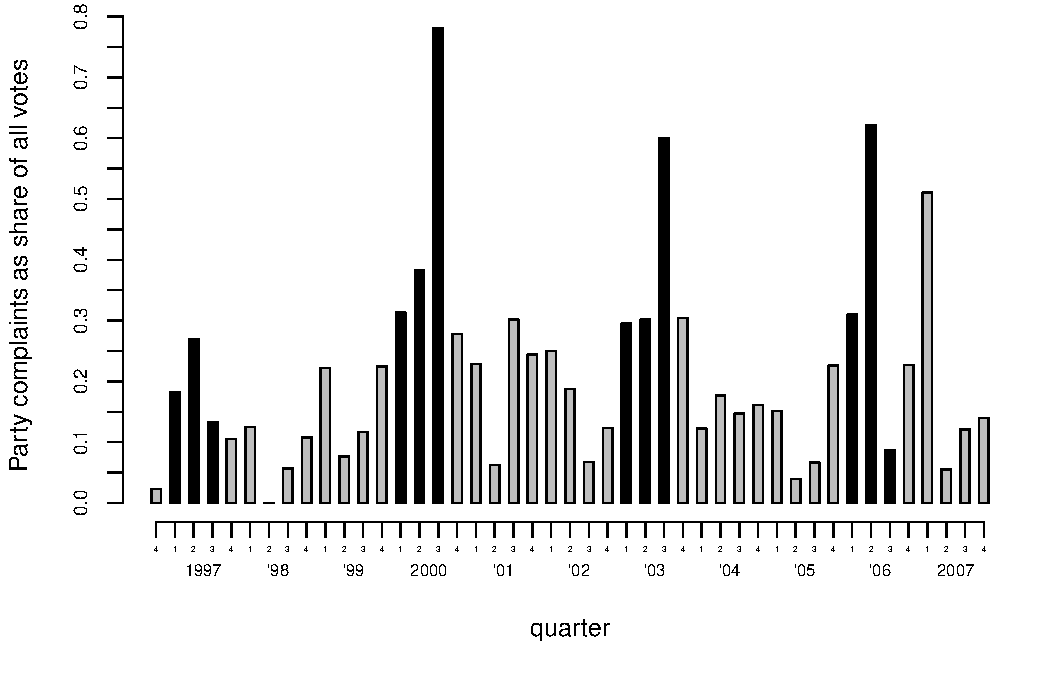
\includegraphics[width=.8\textwidth]{../../graphs/sharePtyComplaintsQuarter.pdf}
 \caption{\emph{Variation in agenda control, 1996--2007.} Party complaints filed at Council General relative to all issues voted. Black bars cover electoral quarters and the immediately previous and next. Data for issue classification provided by Omar Alejandre.}\label{F:agendaControl}
 \end{center}
\end{figure}

As shown in Figure \ref{F:agendaControl}, the complaints filed by parties as a share of all issues considered by the Council General rose steeply in the quarters surrounding every federal election between 1997 and 2007.\footnote{We relied on Omar Alejandre's data to produce this differential for a subset of the period we analyze.}  We define an election cycle as the electoral and immediate previous and next quarters, in which the proportion of party complaints is two-and-a-quarter times higher than in non-electoral periods.  Consistent with our previous discussion, we speculate that the interaction between principals and agents is different in electoral and non-electoral times. Principals (i.e., parties) not only register more complaints in IFE during electoral periods, but we also expect that these complaints will more likely reveal operational preferences and cleavages segmenting IFE's Council General.

The intuition behind this conjecture is easier to explain by considering non-electoral quarters.  If better gatekeeping reduces observable conflict, then much of what the Council General decides during non-electoral periods concern routine administrative matters that do not necessarily map into the main dimension of conflict that divides party sponsors and, consequently, IFE councilors.  In contrast, we believe that electoral times should bring a flurry of activity that increases the number of politically-consequential matters considered by the Council General. To test this proposition, we show the distribution of the absolute value of discrimination parameters ($\text{signal}_i$s) across electoral and non-electoral quarters. If our conjecture about the importance of increased agent restraint during non-electoral periods holds any water, we should see larger average values of discrimination ($\texttt{signal}$) parameters during electoral quarters.

%% Mar31-2013: VIENE DE ifedyn02
\begin{table}
 \begin{center}
   \begin{tabular}{clcc}
     &                        &  Mean & Std.\ dev. \\ \hline
    \mc{4}{c}{Posterior $|x_{j,t}-x_{j,t-1}|$}   \\
    a& New Congress semesters & .140  &   .115    \\
    b& Rest                   & .108  &   .084    \\
%    c& Test a>b (Wilcoxon)    & \mc{2}{c}{$p<.0001$} \\ \hline
    c& Prob.\ a>b             & \mc{2}{c}{.560} \\ \hline
    \mc{4}{c}{Posterior $|\texttt{signal}_i|$}   \\
    d& Electoral quarters     & 2.677 & 1.682  \\ % updated Apr1
    e& Rest                   & 2.601 & 1.684  \\ % updated Apr1
    f& Rest (incl.\ inaugural)& 2.595 & 1.682  \\ % updated Apr1
%    h& Test d>e (Wilcoxon)    & \mc{2}{c}{$p<.0001$} \\ \hline
    g& Prob.\ d>e             & \mc{2}{c}{.565} \\ \hline %% �Como demonios obtuve esto antes? Num. Asimetrico de items
    \mc{4}{c}{Posterior  $\texttt{signal}_i$s with .95 credible ranges off zero} \\
    h& Percentage electoral quarters  & \mc{2}{c}{53\%~~(n=146)} \\ % updated Apr1
    i& Percentage rest                & \mc{2}{c}{45\% (n=1318)}\\ \hline % updated Apr1
    \mc{4}{c}{Abstention rates}   \\
    j& PAN electoral quarter  & \mc{2}{c}{2.1\%~~(n=146)}  \\ % updated Apr2
    k& PAN rest               & \mc{2}{c}{4.6\% (n=1318)}  \\ % updated Apr2
    l& PRI electoral quarter  & \mc{2}{c}{1.0\%~~(n=146)}  \\ % updated Apr2
    m& PRI rest               & \mc{2}{c}{4.1\% (n=1318)}  \\ % updated Apr2
    n& PRD electoral quarter  & \mc{2}{c}{4.5\%~~(n=146)}  \\ % updated Apr2
    o& PRD rest               & \mc{2}{c}{7.2\% (n=1318)}  \\ \hline
   \end{tabular}
  \caption{\emph{Statistics and tests.} See text.}\label{T:tests}
 \end{center}
\end{table}

Rows d and e of Table \ref{T:tests} show the mean and standard deviation of the marginal posterior distribution of absolute discrimination parameters. We proceeded as before by dividing the pooled series into electoral quarters ($n=18$) and not ($n=46$). We dropped the first quarter of each fully-new Council, since these are heavily influenced by our informative priors on ideal points (but report differentials for the full sample in row f). As can be seen from the table, discrimination parameters corresponding to items voted during electoral quarters tend to be larger on average than for the rest. And even if dispersion in the distribution of discrimination parameters is relatively large, it is quite constant across groups of items, letting differences in means stand out.  In fact, a comparison of how often the .95 credible interval of $\texttt{signal}_i$ excludes zero when cases are heard in an electoral as opposed to a non-electoral quarter (rows h and i of Table \ref{T:tests}, respectively) suggests that the cases heard when IFE suffers a loss of agenda control are more likely to be divisive.

%This differential can be exploited in seeking agenda-control effects in voting patterns and, more specifically, party sponsor effects on councilors, contingents and the council as a whole. We hypothesize that the interaction between principals and agents is different in electoral and non-electoral periods. Parties not only register more complaints in election season, but this flurry of party maneuvers increases the number of controversial and politically-consequential matters considered by IFE. Their complaints should provoke greater partisan segmentation of the Council General than in non-electoral periods. Specifically, since party sponsors are likely to bring more pressure to bear upon their councilors during electoral periods, we expect same-sponsor councilors to be more cohesive (i.e., their revealed ideal points to be closer) during electoral cycles. Because party rivalries are likely to be more intense during electoral cycles, we also expect polarization between partisan segments on the council to increase in those periods.

\subsection{Contingent coherence and cross-bloc polarization in electoral quarters}

We can leverage the Council General's cyclical loss of agenda control to derive two additional testable implications of the party watchdog model. Because parties should bring more pressure to bear on their sponsored councilors during electoral periods, we expect same-sponsor contingents to be more cohesive (i.e., their revealed ideal points to be closer) during electoral than non-electoral quarters.  Because party divides should be more notable during electoral periods, we also expect between-party polarization to increase during electoral quarters.  Finally, we believe that party pressure over councilors during electoral quarters should lead to a drop in abstentions during electoral periods, as principals expect from their sponsored councilors a fuller commitment to the defense of their interests.  

We gauge within-contingent cohesion by looking at the posterior marginal distribution of the distance between the most leftist and most rightist councilors within each partisan contingent.\footnote{For the sake of simplicity, we refer to PRI/Green-sponsored councilors as the PRI contingent. The Greens have been in electoral and legislative alliance with the PRI since 2001, and it is reasonable to view their lone IFE member as a case of co-sponsorship.}  We measure between-contingent polarization by looking at the posterior marginal distribution of the distance between the centroids of all pairs of partisan contingents, where the centroids are alternatively defined as the median or average ideological position of the contingents. Abstention rates are the share of within-contingent abstentions in a given quarter. Because we pool posterior samples for periods I--II and III--VII, the spaces have different scales (a .5 shift is small in the latter but not in the former), and these coordinates are arbitrary, we opted to report statistics for standardized ideal point estimates. We therefore subtracted the mean from the posterior ideal point sample and divided it by the standard deviation. 

%We estimate within-contingent polarization with the quarterly posterior marginal distribution of the distance between the councilors farthest apart in each partisan contingent.\footnote{For the sake of simplicity, we refer to PRI/Green-sponsored councilors as the PRI contingent. The Greens have been in electoral and legislative alliance with the PRI since 2001, and it is reasonable to view their lone IFE member as a case of co-sponsorship.}  We estimate between-contingent polarization with the quarterly posterior marginal distribution of the distance between the centroids of all pairs of partisan contingents, where the centroids are defined as the median ideological position among same-sponsor councilors (or mean position in the case of two-member contingents). Between-contingent measures necessitate pairs of multi-member contingents, so quarters where the PRD was either absent from or had a single representative at IFE were excluded from analysis. 

\begin{table}
 \begin{center}
  \begin{tabular}{llrrrrr}
 \hline
                  &  & \mc{2}{c}{Electoral} &  \mc{2}{c}{Non-electoral} & \\
                  &  & \mc{2}{c}{quarter}  &  \mc{2}{c}{quarter}        & \\
                  &  &   \mc{1}{c}{(a)}  &  \mc{1}{c}{(b)}  &  \mc{1}{c}{(c)}  &  \mc{1}{c}{(d)}  & \mc{1}{c}{(e)}  \\
                  &  & Mean      & S.dev.        & Mean    & S.dev. & $\text{Pr}[a<c]$        \\ \hline
   \mc{7}{c}{Within-contingent distances}  \\
   PAN            &  &  0.902 & 0.861 & 1.106 & 0.882 &  0.575  \\
   PRI            &  &  0.863 & 0.562 & 1.278 & 0.982 &  0.605  \\
   PRD$^\dagger$    &  &  2.374 & 1.300 & 1.921 & 1.022 &  0.373    \\ \hline
   \mc{7}{c}{Between-contingent distances}  \\
   PAN-PRI         & &  1.012 & 0.616 & 0.890 & 0.619 &  0.441 \\
   PAN-PRD$^\dagger$ & &  0.475 & 0.372 & 0.637 & 0.515 &  0.572   \\
   PRI-PRD$^\dagger$ & &  1.233 & 0.428 & 1.323 & 0.492 &  0.552   \\ \hline
  \end{tabular}
  \caption{\emph{Election calendar effects on council voting.} Posterior marginal mean and standard deviation of within-contingent and between-contingent polarization (coordinates standardized to make spaces in Figures \ref{F:spaghettis2}a and \ref{F:spaghettis2}b more comparable). $\dagger$ These statistics exclude quarters where no multi-member left contingent was present in the Council General.}\label{t:WiAndBtw}
 \end{center}
\end{table}

Table \ref{t:WiAndBtw} displays statistics for these hypotheses.  Since they are heavily influenced by our semi-informative priors on extremists' ideal points, the first quarters of the Woldenberg and Ugalde councils are dropped before estimating the posterior marginal distribution of these statistics.  The same goes for quarters where a party has fewer than two sponsored councilors (the PRD between the fourth quarter of 2003 and the third of 2008). A glance at the table shows some evidence supporting the hypothesis that within-contingent cohesion increases during the electoral cycle. For all contingents, cohesion is higher (i.e., we observe smaller posterior mean distances) during electoral periods, but posterior standard deviations are generally large. The effect is substantially more important for the PAN- and PRI-, but not for the Left-sponsored contingents. We estimate the probability that cohesion within the PAN and PRI contingents decreases in election season to approach 0.58 and 0.61, respectively (column e of Table \ref{t:WiAndBtw}). For the Left it barely surpasses 0.37. In short, we can weakly substantiate the hypothesis that partisan contingents are more cohesive around election time for two parties only.
\gr{Need to drop freshman quarters from Tab \ref{t:WiAndBtw} in manyDynGraphs.r. Need to run continuous (regression) test for vote-by-vote estimates.}

The evidence for the implication of increased polarization between contingents in electoral periods is yet more scant. Only the PAN and PRI contingents manifested signs of increased polarization, whereas the other two dyads experienced the opposite trend. In terms of probability, the quantity in column a of Table \ref{t:WiAndBtw} should not often be smaller than that in column c. Although margins remain comparable in absolute size to those discussed in the last paragraph, posterior simulations indicate the contrary is likelier for the PAN-PRD and PRI-PRD dyads. 

%To discuss these results, we actually distinguish between the two councils, since the lack of Left-sponsored councilors in the Ugalde years means that the dynamics of polarization between the PRI and the PAN segments are likely to be different across councils.  In any case, polarization increases especially for the PRI-PAN dyad in both councils. The distance between the centroids of each segment, our indicator of polarization, increases about 70\% in both councils. In short, the chances that the PRI contingent will vote with the PAN contingent during electoral periods are lower than during non-electoral quarters.  During the Woldenberg years, the mean distance between the PRI and the PRD contingents was about three times larger than the distance between PRI and PAN contingents.  However, these distances do not wax and wane following the election calendar.  Finally for the PAN-PRD dyad, results indicate smaller mean distances between these sponsors' contingents in election periods (results which visual inspection of maps of the Vald\'es council would indicate are being replicated again).

This last finding concerning less polarization in the PAN-PRD dyad on the council in election season is not trivial, although at face value it refutes the party sponsorship hypothesis with respect to polarization.  A recent study by M\'arquez and Aparicio \citeyearpar{marquez.aparicio.2010} presents the average partisan profile of congressional districts in Mexico from 1997 to 2009 using vote shares of the three-party total adjusted for districting changes in 2006.  Disaggregating their numbers, less than one in ten districts are multi-partisan in their competitive dynamics and about a third of the total are safe bastions for the three major parties (with the PRI well ahead of its two rivals).  The remainder are competitive districts, with victory margins within the average district-level volatility index (about 15 percent of the total vote).  In this group of districts, the dominant pattern of competition is between the PRI and either of its rivals; there are only a dozen or so districts in which the PAN competes directly against the PRD for dominance.  This map is likely repeated in state-level competition, in gubernatorial contests and senatorial contests, and even in municipal races.  What this pattern of competition between dyads suggests is that the PAN and the PRD continue to share long-term strategic interests in their geographically separate contests with the PRI, notwithstanding their bitter presidential contest in 2006. And their agents at IFE reflect these common strategic interests in the rules applied to electoral competition through decisions reached on the council in the midst of election battles.   While anti-PRI convergence at IFE is rarely decisive or stable, it remains a constant feature in the conflicts that arise within the Council General.  Interpreted more generously as a statement of changing intensity in political conflict, the periodic appearance of an anti-PRI coalition during electoral quarters supports the party sponsorship hypothesis and the tripartite segmentation of ideal points when all relevant parties are represented on the council.

%Selection errors
%
%The risk involved in delegation to experts is that of potential agency losses when agents act against the interests of their principals.  The classic solution for minimizing agency costs combines careful screening with permanent monitoring and credible recourse to sanctions in case of non-compliance by agents.  In appointing their agents, principals often stack the deck in favor of compliance from the outset, choosing types with policy predispositions similar to their own \citep{mcnollgast.1987}. To the extent that agents value their jobs and their future, overt as well as implicit threats to use the ``big club behind the door'' \citep{weingast.1984} should reduce any gap in preferences remaining between agents and their principals.  This view of delegation is encapsulated in Mayhew's \citeyearpar{mayhew.1974} seminal model of representatives as automatons concerned only with keeping their constituents happy. A member's revealed preferences, from this viewpoint, will shift only in response to changes in principals' interests.
%
%Of course, selection errors are always possible if improbable.  IFE has presented two clear cases of unexpected mistakes in councilor selection --- two out of 26 councilors appointed since 1997. The first was that of Barrag\'an who for four years occupied the northern extreme of the Woldenberg council, routinely opposed to the other members of the Left contingent, yet faced no threat to his survival. The second example was that of Morales, promoted in 2003 to the council by the PAN, who was consistently opposed to his colleagues sponsored by the same party and well to his south.  Morales met a different fate from Barrag\'an's and was ousted in the first wave of dismissals from the Ugalde council after the 2007 election reform. He was accompanied by PRI-sponsored colleagues Ugalde and Latap\'i, who as nominees of the (losing) Gordillo faction in the power struggles waged by the PRI hierarchy, occupied adjacent but distant positions to the rest of their contingent (see Figures \ref{F:allwMedian}a and \ref{F:allwMedian}b for the combined trajectories of all councilors since 1997).
%
%The demise of the Ugalde council in the wake of the 2007 reform brings to the fore the nuclear option that legislative parties can deploy against IFE's council.  Since IFE's establishment in 1990, four complete sets of councilors have been selected by Congress (in 1990, 1994, 1996 and 2003).  Of these four sets, two have suffered abrupt and total replacement and another has had two thirds of its membership prematurely ousted.  Only the Woldenberg council remained unscathed by congressional interference in councilors' tenure, although impeachment threats were frequently voiced by more than one party's leaders and spokespersons. The not so unusual resort to the nuclear option is the final, ex post instrument used to cow IFE councilors into alignment with their party sponsors.
%
%Esto lo escribi\'o Federico recientemente. 
%1)  No hay errores de selecci\'on.  Claramente falsa, pero nos incumbe establecer exactamente cu\'antos errores se han dado, contextualizarlos y llegar a un n\'umero depurado.  Barrag\'an es un error respecto de su comportamiento en Wold 1, pero no en Wold 2, aunque su selecci\'on igual y obedeci\'o a su reputaci\'on jalisciense de ciudadano "independiente" medio contreras al PRI y al PAN en su estado natal.  Luken es un caso de copatrocinio imprevisto, dado su acercamiento al PRD despu\'es de que el PAN lo nombrara a la lista de suplentes en 1996, m\'as que un caso de error.  Morales es un error, pero habr\'ia que contextualizarlo.  Cuando el PAN lo llev\'o al IEDF, se comport\'o como parte del contingente panista (seg\'un el mapa de una tesina que tengo por ah\'i) -- al igual que el solitario pri\'ista en el consejo local de aquel entonces.  Sospecho que eran todos anti-pejistas.  El pero con Morales es que provino del grupo de Jorge Alcocer (Voz y Voto), m\'as cercano al PRI que al PAN -- Alcocer fue subsecretario con Carpizo, luego a\~nos despu\'es (en los relevos post-Ugalde) ser\'ia apoyado por el PRI para llegar al C.G., pero vetado por el PRD y tambi\'en (creo) por el PAN.  En fin, el error del PAN respecto de Morales fue creer que su anti-pejismo indicaba una inclinaci\'on panista.  Por \'ultimo, los casos de Ugalde y Latap\'i no fueron errores sino efectos de la divisi\'on pri\'ista a partir de 2003 (y la idea de cuotas faccionales se ve apoyada por el dilema actual en el IEDF y el reclamo de los Bejaranistas de su derecho a sponsorship del \'ultimo consejero a nombrarse en estos d\'ias o semanas).  No s\'e c\'omo se ver\'an los 3 m\'as recientes consejeros de Vald\'es hasta tener los mapas est\'aticos actualizados, pero en principio solamente Vald\'es ser\'ia candidato al estatus de "error".  En suma, dos (pero quiz\'as hasta tres) errores en la selecci\'on de un total de 29 consejeros desde 1996.  Menor proporci\'on que la de mariscales de campo fallidos "drafted" en primera ronda en la NFL a lo largo de muchos m\'as a\~nos. 
%
%Para los partidos, en casos de error o drift de a deveras u oportunismo electoral, "Once burned, twice shy". 
%a)  Ya hemos escrito sobre "party capture" y "future rewards" como incentivos a la alineaci\'on de los consejeros con sus sponsors.  Pero no hemos dicho mucho sobre "future punishments".  Es llamativo que el PRI no ha premiado a los miembros "desleales" de su contingente bajo Woldenberg -- Pepe, Merino, Peschard y Rivera (este \'ultimo intent\'o regresar al IFE post-Ugalde, pero fue ignorado por completo por el PRI; Peschard se fue con el PAN al IFAI). Tampoco a Ugalde y Latap\'i (otros dos "desleales" que fueron los primeros desechados del consejo de Ugalde) ni a Morales (no obstante su alineaci\'on con el contingente del PRI, fue promovido por el PAN desde el IEDF y, por tanto, no confiable -- sigue en Voz y Voto desde su relevo).  L\'opez Flores estuvo all over the place y est\'a olvidada por el PRI.  Solamente Virgilio ha sido premiado.  Por el lado del PAN, Molinar y Lujambio fueron super-premiados; Luken alcanz\'o una diputaci\'on local en Baja California, pero fue exclu\'ido de la primaria panista para gobernador este a\~no.  Que sepa, nada ha pasado con Albo y Glez. Luna; pero Arturo S\'anchez es asesor de la dirigencia del PAN actualmente.  Y Morales el desleal fue destituido en la primera ronda del relevo del consejo de Ugalde.  En cuanto al PRD, Barrag\'an ha sufrido el olvido, Zebad\'ua y C\'ardenas fueron promovidos, y Cant\'u fue defendido para C. presidente en 2003 a tal grado que el PRD qued\'o excluido del C.G.  "Future punishments" importan, pues, al mismo grado que "future rewards".
%b)  Y si el margen de error y drift parece demasiado grande, intolerable, para los partidos, siempre queda el \'ultimo recurso de la opci\'on nuclear:  renovaci\'on del C.G. y/o reforma de la ley electoral.  Esto ya lo tenemos hecho.


\section{Conclusion}
\label{S:conclusion}

(Forthcoming.) 

\gr{Cuadratic kernel window? Discuss drop of non-council members from estimation, handling asymmteric matrices. Selection errors. New Congress effects.}




\begin{singlespace}

\bibliographystyle{apsr}
%\bibliography{D:/01/Dropbox/mydocs/magar}
\bibliography{/home/eric/Dropbox/mydocs/magar}
%\bibliography{../../mydocs/magar}

\end{singlespace}


\end{document}
